\chapter{DDD}

\section{Giới thiệu về thiết kế hướng miền (Domain Driven Design)}

Thiết kế hướng miền được Eric Evans giới thiệu trong cuốn sách \emph{"Domain Driven Design: Tackling Complexity in the Heart of Software"}. \emph{Thiết kế hướng miền (Domain Driven Design)} là một hướng tiếp cận thiết kế phần mềm tập trung vào việc hiểu rõ và mô hình hóa lĩnh vực kinh doanh của một tổ chức. Thiết kế hướng miền nhấn mạnh việc sử dụng lĩnh vực nghiệp vụ kinh doanh để thảo luận và đề xuất giải pháp đáp ứng nhu cầu.

Hệ thống phần mềm được tạo ra để xử lý công việc trong cuộc sống hiện đại. Việc phát triển hệ thống liên kết chặt chẽ với một số khía cạnh cụ thể trong cuộc sống của chúng ta. Trong thiết kế hướng miền, \emph{miền (Domain)} đề cập đến phạm vi kiến thức và vấn đề cụ thể mà hệ thống xử lý.

\begin{itemize}

\item Về góc độ kinh doanh: Miền đại diện cho một lĩnh vực hoặc ngành mà doanh nghiệp hoạt động.

\item Về góc độ hệ thống: Miền có thể coi là đại diện cho không gian vấn đề của hệ thống.

\end{itemize}

\begin{example} \emph{Trong đồ án này, miền được xác định là bài toán giải pháp hóa đơn điện tử.}

\end{example}

Với nhiều phần mềm thiết kế không tốt, phần xử lý các công việc không liên quan đến vấn đề nghiệp vụ kinh doanh như truy cập tập tin, hạ tầng mạng, cơ sở dữ liệu, \dots được lập trình trong đối tượng nghiệp vụ kinh doanh. Cách này giúp tốc độ hoàn thiện nhanh. Tuy nhiên, cách này làm dự án bị mất đi tính hướng đối tượng khó thay thay đổi, mở rộng hệ thống,\dots Thiết kế hướng miền cung cấp một cách để tổ chức mã nguồn và dễ dàng thích ứng với các yêu cầu thay đổi.

Trong kiến trúc vi dịch vụ, thiết kế hướng miền đảm bảo mỗi dịch vụ được thiết kế phản ánh một phần cụ thể của lĩnh vực kinh doanh. Mỗi dịch vụ được quản lí bởi một nhóm phát triển được hỗ trợ bởi các chuyên gia ngành. Trong thiết kế hướng miền, \emph{chuyên gia ngành (Domain Expert)} là người có kiến thức và hiểu biết sâu sắc về vấn đề đang được hệ thống phần mềm giải quyết. Chuyên gia ngành thể hiện chính xác vấn đề kinh doanh, đóng vai trò là nguồn thông tin cho nhóm phát triển.

\section{Cốt lõi của thiết kế hướng miền}

% Giới thiệu về các mẫu chiến lược và các mẫu kỹ thuật

Thiết kế hướng miền cung cấp 2 loại mẫu:

\begin{itemize}

\item \emph{Các mẫu chiến lược (Strategic Patterns):} Phân chia một miền lớn và phức tạp thành các phần nhỏ hơn với ranh giới được xác định rõ ràng. Giúp phân chia một miền lớn hợp lý.

\item \emph{Các mẫu kỹ thuật (Tactical Patterns):} Hiện thực hóa các khái niệm và qui trình trong thành phần thành các thiết kế hệ thống phần mềm. Giúp hệ thống phù hợp với kinh doanh.

\end{itemize}

\begin{figure}[H]

\centering

\includegraphics[scale = 0.5]{pictures/cac_mau_chien_luoc_va_cac_mau_ky_thuat/main.drawio.png}

\caption{Tổng quan về Strategic Patterns và Tactical Patterns}

\end{figure}

Thiết kế hướng miền cung cấp 2 loại mẫu:

\begin{itemize}

\item \emph{Các mẫu chiến lược (Strategic Patterns):} Phân chia một miền lớn và phức tạp thành các phần nhỏ hơn với ranh giới được xác định rõ ràng. Giúp phân chia một miền lớn hợp lý.

\item \emph{Các mẫu kỹ thuật (Tactical Patterns):} Hiện thực hóa các khái niệm và qui trình trong thành phần thành các thiết kế hệ thống phần mềm. Giúp hệ thống phù hợp với kinh doanh.

\end{itemize}

\begin{figure}[H]

\centering

\includegraphics[scale = 0.5]{pictures/cac_mau_chien_luoc_va_cac_mau_ky_thuat/main.drawio.png}

\caption{Tổng quan về Strategic Patterns và Tactical Patterns}

\end{figure}

% \subsection{Chi tiết về các mẫu chiến lược và các mẫu kỹ thuật}

\section{Các mẫu chiến lược của thiết kế hướng miền}

% \chapter{Các mẫu chiến lược}

Các mẫu chiến lược phân tích nghiệp vụ kinh doanh sau đó đưa ra việc phân chia các thành phần và hiểu mối quan hệ của các thành phần đó. Từ đó, các mẫu chiến lược giúp xác định các thành phần quan trọng của hệ thống, đảm bảo kiến trúc phần mềm phản ánh đúng các yêu cầu kinh doanh. Từ việc phân chia hệ thống thành các thành phần nhỏ, chúng ta có thể tạo ra hệ thống mở rộng dễ dàng, phát triển linh hoạt theo nhu cầu kinh doanh.

Các mẫu chiến lược bao gồm:

\begin{itemize}

% các mục nhỏ ben dưới

% các mục nhỏ ben dưới

% các mục nhỏ ben dưới

% các mục nhỏ ben dưới

% các mục nhỏ ben dưới

% các mục nhỏ ben dưới

\item Muc1

\item Muc2

\item Muc1

\item Muc2

\item Muc1

\item Muc2

\item Muc1

\item Muc2

\end{itemize}

% nội dung trang lớn lên để hết giấy

% nội dung trang lớn lên để hết giấy

% nội dung trang lớn lên để hết giấy

% nội dung trang lớn lên để hết giấy

% nội dung trang lớn lên để hết giấy

\begin{figure}[H]

\centering

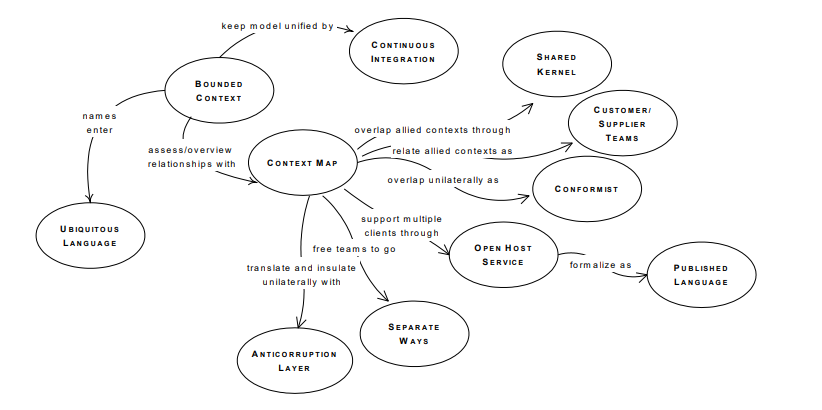
\includegraphics[scale = 0.9]{pictures/cac_mau_chien_luoc/temp.png}

\caption{Sơ đồ về các thành phần trong mô hình chiến lược}

\end{figure}

%!<! - - $ Vẽ lại sau: - - >

%!<! - - $ Vẽ lại sau: - - >

%!<! - - $ Vẽ lại sau: - - >

%!<! - - $ Vẽ lại sau: - - >

%!<! - - $ Vẽ lại sau: - - >

%!<! - - $ Vẽ lại sau: - - >

%!<! - - $ Vẽ lại sau: - - >

%!<! - - $ Vẽ lại sau: - - >

%!<! - - $ Vẽ lại sau: - - >

%!<! - - $ Vẽ lại sau: - - >

% \section{Miền phụ (Sub - Domain)}

Một miền lớn được tạo thành từ nhiều \emph{miền phụ (Sub - Domain)}. Trong thực tế, một miền kinh doanh phức tạp không thể có một chuyên gia ngành có kiến thức về tất cả các miền phụ.

\begin{example} Trong miền thương mại điện tử lớn có thể có một số miền phụ sau:

\begin{itemize}

\item \textbf{Miền phụ quản lý hàng tồn kho:} liên quan đến việc quản lý sản phẩm trong kho hàng.

\item \textbf{Miền phụ quản lý khách hàng:} liên quan đến việc quản lý tài khoản khách hàng.

\item \textbf{Miền phụ vận chuyển:} liên quan đến việc quản lý việc vận chuyển giao hàng.

\end{itemize}

\end{example}

% \subsection{Phân loại các miền phụ}

Trong thiết kế hướng miền, có ba loại miền phụ là:

\begin{itemize}

\item Miền phụ chung (Generic Subdomain)

\item Miền phụ cốt lõi (Core Subdomain)

\item Miền phụ hỗ trợ (Supporting Subdomain)

\end{itemize}

% \subsubsection{Miền phụ chung (Generic Subdomain)}

Miền phụ chung cung cấp các giải pháp có sẵn mà doanh nghiệp có thể mua. Miền phụ chung có thể được tìm thấy trên nhiều ngành. Doanh nghiệp không thể đạt được bất kỳ lợi thế cạnh tranh nào so với đối thủ bằng cách thực hiện những điều khác biệt trong miền phụ chung.

\begin{example} Các miền phụ chung \textit{"quản lý nhân sự"} hay \textit{"quản lý cơ sở vật chất"} không tạo thêm bất kỳ giá trị khác biệt nào cho doanh nghiệp.

\end{example}

% \subsubsection{Miền phụ cốt lõi (Core Subdomain)}

Miền phụ cốt lõi là phần quan trọng và có giá trị nhất của hệ thống. Miền phụ cốt lõi giúp phân biệt các doanh nghiệp và làm cho các doanh nghiệp có giá trị. Miền phụ cốt lõi tập trung vào mục tiêu và yêu cầu của khách hàng với doanh nghiệp, từ đó quyết định sự thành công của doanh nghiệp. Vì vậy, mỗi doanh nghiệp luôn tìm cách thực hiện những điều khác biệt trong các miền phụ cốt lõi này để đạt được lợi thế so với đối thủ cạnh tranh.

\begin{example} Trong miền thẻ tín dụng, miền phụ cốt lõi có thể là \textit{"phát hành thẻ"} chịu trách nhiệm về quá trình phát hành thẻ tín dụng cho khách hàng. Miền phụ cốt lõi này bao gồm các nhiệm vụ như: thu thập thông tin khách hàng, thực hiện kiểm tra tín dụng, kích hoạt thẻ, \dots

\end{example}

% \subsubsection{Miền phụ hỗ trợ (Supporting Subdomain)}

Các miền phụ cốt lõi phụ thuộc vào các miền phụ hỗ trợ. Miền phụ hỗ trợ cung cấp các dịch vụ để miền phụ cốt lõi hoạt động hiệu quả. Tuy nhiên, miền phụ hỗ trợ không đòi hỏi mức độ phức tạp cao về logic nghiệp vụ.

\begin{example} Trong nhiều phần mềm, miền phụ hỗ trợ \textit{"xác thực người dùng"} OAuth 2.0 của Facebook hoặc Google hỗ trợ cho miền phụ cốt lõi hoạt động hiệu quả.

\end{example}

% \subsection{Cách xác định các miền phụ}

Các miền phụ cốt lõi, hỗ trợ và chung có thể khác nhau đối với các doanh nghiệp hoạt động trong cùng một miền. Vì các miền phụ được xác định tùy theo nhu cầu kinh doanh và bối cảnh cụ thể của mỗi tổ chức.

\subsubsection{Mô tả cách xác định các miền phụ}

\begin{enumerate}

\item Bắt đầu bằng cách xem xét nghiệp vụ kinh doanh.

\item Nếu có sẵn giải pháp đã biết thì có khả năng là miền phụ chung. Ngược lại, chúng ta kiểm tra nghiệp vụ kinh doanh đó có thêm giá trị kinh doanh nào hay không?

\item Nếu không có giá trị kinh doanh thì chúng ta kiểm tra xem các miền phụ cốt lõi có phụ thuộc vào miền phụ này hay không? Nếu có thì có khả năng là miền phụ hỗ trợ. Nếu không thì đó là miền phụ chung.

\item Nếu miền phụ có tiềm năng bổ sung một số giá trị kinh doanh thì bước kiểm tra tiếp theo là xem liệu miền doanh nghiệp có độ phức tạp cao hay không?

\item Nếu miền doanh nghiệp không có độ phức tạp cao thì có khả năng là miền phụ hỗ trợ. Ngược lại thì nó có khả năng là miền phụ cốt lõi.

\end{enumerate}

\begin{figure}[h]

\centering

\includegraphics[scale = 0.5]{pictures/cach_xac_dinh_cac_mien_phu/main.drawio.png}

\caption{Sơ đồ xác định các miền phụ}

\end{figure}

% \subsection{Áp dụng phân loại miền phụ trong đồ án này}

% %!<! - - Hướng dẫn: 5/3 - - >

% %!<! - - Hướng dẫn: 5/3 - - >

% %!<! - - Hướng dẫn: 5/3 - - >

% %!<! - - Hướng dẫn: 5/3 - - >

% %!<! - - Hướng dẫn: 5/3 - - >

% %!<! - - Hướng dẫn: 5/3 - - >

% %!<! - - Hướng dẫn: 5/3 - - >

% %!<! - - Hướng dẫn: 5/3 - - >

% %!<! - - Hướng dẫn: 5/3 - - >

% %!<! - - Hướng dẫn: 5/3 - - >

% %!<! - - Hướng dẫn: 5/3 - - >

% %!<! - - Hướng dẫn: 5/3 - - >

% %!<! - - Hướng dẫn: 5/3 - - >

% %!<! - - Hướng dẫn: 5/3 - - >

% %!<! - - Hướng dẫn: 5/3 - - >

% %!<! - - Hướng dẫn: 5/3 - - >

% ChatGPT?

% Ứng dụng thiết kế hướng miền với hóa đơn điện tử thì miền phụ hỗ trợ có thể là gì?

\subsubsection{Áp dụng phân loại miền phụ trong đồ án này}

\subsubsection{Áp dụng phân loại miền phụ trong đồ án này}

\subsubsection{Áp dụng phân loại miền phụ trong đồ án này}

\subsubsection{Áp dụng phân loại miền phụ trong đồ án này}

\subsubsection{Áp dụng phân loại miền phụ trong đồ án này}

\subsubsection{Áp dụng phân loại miền phụ trong đồ án này}

\subsubsection{Áp dụng phân loại miền phụ trong đồ án này}

\subsubsection{Áp dụng phân loại miền phụ trong đồ án này}

\subsubsection{Áp dụng phân loại miền phụ trong đồ án này}

\subsubsection{Áp dụng phân loại miền phụ trong đồ án này}

\subsubsection{Áp dụng phân loại miền phụ trong đồ án này}

\subsubsection{Áp dụng phân loại miền phụ trong đồ án này}

\subsubsection{Áp dụng phân loại miền phụ trong đồ án này}

\section{Các mẫu kỹ thuật của thiết kế hướng miền}

\section{DDD}

\section{DDD}

\section{DDD}

\section{DDD}

\section{DDD}

% \section{Mô hình miền (Domain Models)}

Để tạo một phần mềm tốt, chúng ta cần phải hiểu rõ về phần mềm đó. Trong thiết kế hướng miền để có thể hiểu miền nhanh, chúng ta cần tạo ra các mô hình miền. Mô hình miền (Domain Models) là kiến thức có tổ chức và có cấu trúc về miền phù hợp để giải quyết vấn đề kinh doanh. Mục tiêu của mô hình miền là cung cấp rõ ràng, ngắn gọn và chính xác về miền làm cơ sở để hệ thống giải quyết vấn đề kinh doanh.

% \begin{example} Trong đồ án này, mô hình miền của em bao gồm các yêu cầu nghiệp vụ và các sơ đồ: UML Use Case Diagrams, UML Class Diagrams,\dots kĩ thuật ở phần sau

% \end{example}

% \section{Bối cảnh bị giới hạn (Bounded Context)}

Một miền cần chia đủ nhỏ để phù hợp với một nhóm cụ thể. Để đạt được điều này, chúng ta cần xác định rõ ranh giới giữa các ngữ cảnh. \emph{Bối cảnh bị giới hạn (Bounded Context)} giúp xác định rõ các ranh giới, chia miền thành các phần độc lập để giải quyết sự phức tạp trong mô hình doanh nghiệp. Bối cảnh bị giới hạn tạo ra các mô hình khác nhau cho các lĩnh vực khác nhau của miền. Bối cảnh bị giới hạn thể hiện phạm vi kinh doanh của dịch vụ.

\begin{figure}[H]

\centering


\includegraphics[scale = 1]{pictures/boi_canh_gioi_han/main.png}

\caption{Ví dụ về bối cảnh bị giới hạn trong một ngân hàng}

\end{figure}

\subsubsection{Cách xác định bối cảnh bị giới hạn}

Để có thể xác định được bối cảnh bị giới hạn chúng ta có thể xem xét:

\begin{itemize}

\item Dựa vào việc phân chia các miền phụ.

\item Dựa vào sơ đồ cấu trúc tổ chức các phòng ban của doanh nghiệp.

\item Dựa vào modules của các ứng dụng kiến trúc nguyên khối (nếu việc phân chia tốt).

\item Dựa vào trách nhiệm và hoạt động của chuyên gia ngành.

\end{itemize}

\subsubsection{Áp dụng xác định bối cảnh bị giới hạn trong đồ án này}

\subsubsection{Áp dụng xác định bối cảnh bị giới hạn trong đồ án này}

\subsubsection{Áp dụng xác định bối cảnh bị giới hạn trong đồ án này}

\subsubsection{Áp dụng xác định bối cảnh bị giới hạn trong đồ án này}

\subsubsection{Áp dụng xác định bối cảnh bị giới hạn trong đồ án này}

\subsubsection{Áp dụng xác định bối cảnh bị giới hạn trong đồ án này}

\subsubsection{Áp dụng xác định bối cảnh bị giới hạn trong đồ án này}

\subsubsection{Áp dụng xác định bối cảnh bị giới hạn trong đồ án này}

\subsubsection{Áp dụng xác định bối cảnh bị giới hạn trong đồ án này}

\subsubsection{Áp dụng xác định bối cảnh bị giới hạn trong đồ án này}

\subsubsection{Áp dụng xác định bối cảnh bị giới hạn trong đồ án này}

\subsubsection{Áp dụng xác định bối cảnh bị giới hạn trong đồ án này}

%!<! - - Hướng dẫn 5/10 - - >

%!<! - - Hướng dẫn 5/10 - - >

%!<! - - Hướng dẫn 5/10 - - >

%!<! - - Hướng dẫn 5/10 - - >

%!<! - - Hướng dẫn 5/10 - - >

%!<! - - Hướng dẫn 5/10 - - >

%!<! - - Hướng dẫn 5/10 - - >

%!<! - - Hướng dẫn 5/10 - - >

%!<! - - Hướng dẫn 5/10 - - >

% \section{Ngôn ngữ chung (Ubiquitous Language)}

Trong quá trình xây dựng mô hình miền, cần có trao đổi giữa người thiết kế hệ thống và chuyên gia ngành để hiểu đúng về miền. Tuy nhiên, nhóm kinh doanh sử dụng ngôn ngữ kinh doanh và nhóm công nghệ có xu hướng sử dụng các thuật ngữ kỹ thuật trong giao tiếp của họ. Người phát triển phần mềm tập trung vào lớp, phương thức, thuật toán, trong khi chuyên gia ngành thường sử dụng ngôn ngữ chuyên ngành của họ. Sự khác biệt về ngôn ngữ giữa các thành viên có thể dẫn đến những thách thức về giao tiếp. Ngoài ra, trong các lĩnh vực kinh doanh khác nhau, một thuật ngữ có thể được sử dụng trong nhiều miền, cùng với ý nghĩa khác nhau gây ra sự nhầm lẫn và hiểu sai cho các người phát triển phần mềm cũng như các chuyên gia ngành.

Thiết kế hướng miền đề xuất sử dụng ngôn ngữ chung để giải quyết những thách thức ngôn ngữ. \emph{Ngôn ngữ chung (Ubiquitous Language)} là một ngôn ngữ được cấu trúc xung quanh mô hình miền và được tất cả các thành viên trong nhóm sử dụng cho mọi hoạt động của nhóm với phần mềm. Ngôn ngữ chung được xác định bởi các từ vựng và có định nghĩa rõ ràng về ngữ cảnh sử dụng từ vựng.

\subsubsection{Một số đặc điểm của ngôn ngữ chung}

\begin{itemize}

\item Ngôn ngữ chung được sử dụng bởi cả chuyên gia ngành và chuyên gia công nghệ.

\item Có nhiều ngôn ngữ chung trong một tổ chức được mỗi nhóm tạo và quản lý một cách độc lập.

\item Việc tạo ra ngôn ngữ chung là một quá trình liên tục. Ngôn ngữ chung phát triển theo thời gian thông qua sự cộng tác giữa doanh nghiệp và các chuyên gia công nghệ.

\item Các thành viên phải sử dụng ngôn ngữ chung cho công việc và trong toàn bộ hệ thống

\end{itemize}

\begin{figure}[H]

\centering


\includegraphics[scale = 0.6]{pictures/ngon_ngu_chung/main.png}

\caption{Ngôn ngữ chung được sử dụng trong toàn bộ hệ thống}

\end{figure}



%@ Tích hợp liên tục

%@ Tích hợp liên tục

%@ Tích hợp liên tục

%@ Tích hợp liên tục

%@ Tích hợp liên tục
%!<! - - @Tích hợp Liên tục (Continuous Integration) - - >

Tích hợp Liên tục (Continuous Integration): là việc các thành viên trong nhóm phát triển tích hợp mã nguồn vào một hệ thống chung thường xuyên. Khi có mã nguồn mới việc tích hợp liên tục sẽ tự động kiểm thử và xây dựng giảm xung đột giữa các phiên bản mã nguồn khác nhau, giúp phát hiện và sửa lỗi sớm hơn.

% CD là gì

% CD là gì

% CD là gì

% CD là gì

% CD là gì

% CD là gì

% CD là gì

% CD là gì

% CD là gì

CI/CD là viết tắt của hai khái niệm quan trọng trong quá trình phát triển phần mềm: Continuous Integration (CI) và Continuous Delivery (CD). Đây là một phương pháp giúp tự động hóa quy trình phát triển, kiểm thử, và triển khai ứng dụng, giúp tăng cường chất lượng phần mềm và giảm thời gian cũng như rủi ro trong quá trình phát triển.

1. **Continuous Integration (CI - Tích hợp liên tục):**

- **Mục tiêu:** Đảm bảo rằng mã nguồn mới được tích hợp vào mã nguồn chính (main codebase) một cách tự động và thường xuyên, giảm thời gian giữa việc viết mã và phát hành.

- **Quy trình:** Mỗi khi một nhà phát triển hoàn thành một tính năng hoặc sửa lỗi, họ tích hợp mã của mình vào mã nguồn chính. Hệ thống CI sẽ tự động kiểm tra mã này bằng cách chạy các bài kiểm thử tự động để đảm bảo rằng nó không làm hỏng hệ thống.

2. **Continuous Delivery (CD - Phân phối liên tục):**

- **Mục tiêu:** Tự động hóa việc triển khai ứng dụng để có thể phân phối bản vá, tính năng hoặc cập nhật một cách nhanh chóng và đáng tin cậy.

- **Quy trình:** Nếu quá trình CI thành công, mã nguồn sẽ được triển khai tự động lên môi trường thử nghiệm (staging environment). Nếu mọi thứ ổn, nó có thể được triển khai tự động lên môi trường sản phẩm (production environment).

3. **Continuous Deployment (CD - Triển khai liên tục):**

- **Khác biệt với Continuous Delivery:** Trong Continuous Deployment, nếu mọi thứ qua bài kiểm thử được tự động và thành công, mã nguồn sẽ tự động triển khai lên môi trường sản phẩm mà không cần sự can thiệp thủ công.

- **Mục tiêu:** Tối ưu hóa quá trình triển khai, giảm thiểu sự chờ đợi và đảm bảo tính ổn định của hệ thống.

4. **Các công cụ thường được sử dụng:**

- **Jenkins, Travis CI, CircleCI:** Đối với CI.

- **Docker, Kubernetes:** Đối với CD, đặc biệt là việc triển khai và quản lý containerized applications.

- **Ansible, Puppet, Chef:** Công cụ tự động hóa cấu hình và triển khai.

Tổng cộng, CI/CD giúp tăng cường khả năng linh hoạt, đảm bảo chất lượng mã nguồn, giảm rủi ro, và giảm thời gian giữa việc phát triển và triển khai sản phẩm.

% CD là gì

% CD là gì

% CD là gì

% CD là gì

% CD là gì

% CD là gì

% CD là gì

% CD là gì

% CD là gì

% CD là gì

Khi một bối cảnh giới hạn đã được xác định, chúng ta cần đảm bảo rằng nó luôn ở trạng thái mới và hoạt động tốt như kỳ vọng. Đáp ứng nhu cầu doanh nghiệp phát triển thay đổi liên tục và nhanh chóng.

Khi cùng vận hành và phát triển xung đột có thể xảy ra ở cùng hoặc khác bối cảnh giới hạn.

= > Vì vậy, cần sử dụng việc tích hợp liên tục tạo ra một quy trình tự động và liên tục từ việc tích hợp mã nguồn, kiểm thử tự động giúp tăng cường chất lượng phần mềm, giảm thời gian và rủi ro trong quá trình phát triển phần mềm.

%!<! - - $VD: jenkins - - >

%!<! - - unit test - - >

%!<! - - test tích hợp - - >

% vở

% thời gian khác nhau

% http://localhost nên không có CD
% \section{Bản đồ bối cảnh (Context Maps)}

Các bối cảnh bị giới hạn phải độc lập trong bối cảnh riêng và có mô hình miền riêng, nhưng các bối cảnh bị giới hạn cần tương tác, giao tiếp để trao đổi thông tin. Vì vậy các bối cảnh bị giới hạn có thể có mối quan hệ với nhau. Những mối quan hệ này cần được quản lý chặt chẽ để hoạt động độc lập, nhất quán và linh hoạt. Do đó, cần phải ghi lại các mối quan hệ thông qua việc sử dụng bản đồ bối cảnh. \emph{Bản đồ bối cảnh (Context Maps)} là sự thể hiện trực quan của hệ thống, thể hiện các thành phần và mối quan hệ giữa các thành phần.

\begin{figure}[H]

\centering

\includegraphics[scale = 0.4]{pictures/ban_do_boi_canh/main.drawio.png}

\caption{Ví dụ bản đồ bối cảnh trong 1 ngân hàng}

\end{figure}

%! Vẽ lại tiếng Việt

%! Vẽ lại tiếng Việt

%! Vẽ lại tiếng Việt

%! Vẽ lại tiếng Việt

%! Vẽ lại tiếng Việt

%! Vẽ lại tiếng Việt

%! Vẽ lại tiếng Việt

%! Vẽ lại tiếng Việt

%! Vẽ lại tiếng Việt

%! Vẽ lại tiếng Việt

% \section{Các mối quan hệ bối cảnh bị giới hạn}

% Có 3 loại mối quan hệ giữa các bối cảnh bị giới hạn là:

\begin{itemize}

\item Mối quan hệ đối xứng (Symmetric Relationship)

\textbf{Mô tả:} Thể hiện sự tương tác 2 chiều giữa 2 bối cảnh bị giới hạn .

\item Mối quan hệ bất đối xứng (Asymmetric Relationship)

\textbf{Mô tả:} Thể hiện sự tương tác 1 chiều giữa 2 các bối cảnh bị giới hạn .

\item Mối quan hệ 1 - nhiều (One to Many Relationship)

\textbf{Mô tả:} Thể hiện sự tương tác 1 chiều giữa 1 bối cảnh bị giới hạn với nhiều bối cảnh bị giới hạn khác.

\end{itemize}

\begin{figure}[H]

\centering


\includegraphics[scale = 0.5]{pictures/cac_moi_quan_he_boi_canh_gioi_han/main.png}

\caption{Các mối quan hệ bối cảnh bị giới hạn}

\end{figure}



%%%%%%%%%%%%%%%%%%%%%%%%%%%%%%%%%%

%%%%%%%%%%%%%%%%%%%%%%%%%%%%%%%%%%

%%%%%%%%%%%%%%%%%%%%%%%%%%%%%%%%%%

%%%%%%%%%%%%%%%%%%%%%%%%%%%%%%%%%%

%%%%%%%%%%%%%%%%%%%%%%%%%%%%%%%%%%

%%%%%%%%%%%%%%%%%%%%%%%%%%%%%%%%%%

%%%%%%%%%%%%%%%%%%%%%%%%%%%%%%%%%%

% \subsection{Mối quan hệ đối xứng (Symmetric Relationship)}

% \subsubsection{Mô hình riêng biệt (Separate Ways)}

% Mô hình riêng biệt (Separate Ways) khi các bối cảnh bị giới hạn có quan hệ riêng biệt, không có sự phụ thuộc. Vì vậy, các bối cảnh bị giới hạn này có ngôn ngữ, mô hình, mục đích độc lập và thực thi riêng biệt. Các nhóm phát triển không phải cộng tác hay phối hợp với nhau từ đó đem lại lợi ích dễ dàng bảo trì và mở rộng hệ thống.

\begin{example} Trong miền vấn đề ngân hàng, thẻ tín dụng và khoản vay mua nhà không có mối quan hệ.

\begin{figure}[H]

\centering

\includegraphics[scale = 0.5]{pictures/mo_hinh_rieng_biet_separate_ways/main.drawio.png}

\caption{Ví dụ mô hình riêng biệt (Separate Ways)}

\end{figure}

\end{example}



% \subsubsection{Mô hình hạt nhân chung (Shared Kernel)}

% Trong thực tế, nhiều bối cảnh bị giới hạn phụ thuộc lẫn nhau. Mô hình hợp tác (Partnership) tạo điều kiện cho việc giao tiếp và cộng tác giữa các bối cảnh bị giới hạn phụ thuộc. Tuy nhiên, sự phụ thuộc này dẫn đến mức độ kết hợp cao giữa các nhóm và bối cảnh bị giới hạn, dẫn tới mất đi tính độc lập.

\textit{Lưu ý: Mô hình hợp tác không phải là mô hình của các mẫu chiến lược trong thiết kế huớng miền.}

Để giải quyết vấn đề bối cảnh bị giới hạn phụ thuộc lẫn nhau chúng ta có mô hình hạt nhân chung. Mô hình hạt nhân chung (Shared Kernel) cho phép các bối cảnh bị giới hạn có phần chia sẻ chung và có ranh giới phân định rõ ràng. Từ đó, tách việc quản lí các mô hình hạt nhân chung này một cách độc lập với phần còn lại của bối cảnh bị giới hạn . Khi cần thay đổi mà không phải của mô hình hạt nhân chung thì nhóm sẽ hoạt động độc lập. Thông thường, mô hình hạt nhân chung được hiện thực hóa bằng các thư viện chung. Tuy nhiên, chỉ sử dụng mô hình hạt nhân chung nếu quan hệ của các bối cảnh bị giới hạn nhỏ và ổn định để tránh quan hệ phức tạp và ràng buộc chặt chẽ.

% Vẽ lại bản đồ tiếng Việt

% Vẽ lại bản đồ tiếng Việt

% Vẽ lại bản đồ tiếng Việt

% Vẽ lại bản đồ tiếng Việt

% Vẽ lại bản đồ tiếng Việt

% Vẽ lại bản đồ tiếng Việt

% Vẽ lại bản đồ tiếng Việt

% Vẽ lại bản đồ tiếng Việt

% Từ bản đồ lấy vi dụ cho các mô hình

% Từ bản đồ lấy vi dụ cho các mô hình

% Từ bản đồ lấy vi dụ cho các mô hình

% Từ bản đồ lấy vi dụ cho các mô hình

% Từ bản đồ lấy vi dụ cho các mô hình

% Từ bản đồ lấy vi dụ cho các mô hình

% Từ bản đồ lấy vi dụ cho các mô hình

% Từ bản đồ lấy vi dụ cho các mô hình

% Từ bản đồ lấy vi dụ cho các mô hình

% Từ bản đồ lấy vi dụ cho các mô hình

\begin{example} Trong miền vấn đề ngân hàng, thẻ tín dụng và khoản vay mua nhà không có mối quan hệ.

\begin{figure}[H]

\centering

\includegraphics[scale = 0.5]{pictures/mo_hinh_rieng_biet_separate_ways/main.drawio.png}

\caption{Ví dụ mô hình riêng biệt (Separate Ways)}

\end{figure}

\end{example}

% %! $VD: hình giao như 2 tập hợp - - >

% \subsection{Mối quan hệ bất đối xứng (Asymmetric Relationship)}

% Trong mối quan hệ bất đối xứng, một bối cảnh bị giới hạn có sự phụ thuộc vào một bối cảnh bị giới hạn khác. Mối quan hệ này được mô tả bằng cách gán vai trò cho bối cảnh bị giới hạn :

\begin{itemize}

\item \textbf{Bối cảnh bị giới hạn thượng nguồn (Upstream):}

\begin{itemize}

\item Bối cảnh bị giới hạn cung cấp cho bối cảnh bị giới hạn khác.

\item Ký hiệu: U

\end{itemize}

\item \textbf{Bối cảnh bị giới hạn hạ lưu (Downstream):}

\begin{itemize}

\item Bối cảnh bị giới hạn phụ thuộc vào bối cảnh bị giới hạn khác.

\item Ký hiệu: D

\end{itemize}

\end{itemize}

\begin{example} Mối quan hệ bất đối xứng giữa bối cảnh bị giới hạn A và bối cảnh bị giới hạn B.

\begin{itemize}

\item Bối cảnh bị giới hạn A ràng buộc với bối cảnh bị giới hạn B

\item Bối cảnh bị giới hạn A đóng vai trò là bối cảnh bị giới hạn hạ lưu (Downstream)

\item Bối cảnh bị giới hạn B đóng vai trò là bối cảnh bị giới hạn thượng nguồn (Upstream)

\item Bối cảnh bị giới hạn A có kiến thức về các mô hình trong bối cảnh bị giới hạn B

\item Bối cảnh bị giới hạn B không có bất kỳ kiến thức nào về mô hình trong bối cảnh bị giới hạn A

\end{itemize}

\begin{figure}[H]

\centering

\includegraphics[scale = 0.5]{pictures/moi_quan_he_bat_doi_xung/main.drawio.png}

\caption{Ví dụ mối quan hệ bất đối xứng}

\end{figure}

\end{example}

% \subsubsection{Mô hình khách hàng - nhà cung cấp (Customer - Supplier)}

% Mô hình khách hàng - nhà cung cấp (Customer - Supplier) được thể hiện rằng bối cảnh bị giới hạn thượng nguồn đáp ứng nhu cầu của bối cảnh bị giới hạn hạ lưu.

Khi đó:

\begin{itemize}

\item Bối cảnh bị giới hạn thượng nguồn được gọi là nhà cung cấp.

\item Bối cảnh bị giới hạn hạ lưu được gọi là khách hàng.

\end{itemize}

Trong thực tế, nhóm phát triển nhà cung cấp luôn tham khảo ý kiến của nhóm phát triển khách hàng và có bộ kiểm thử để đảm bảo rằng dịch vụ của nhà cung cấp đáp ứng được yêu cầu của khách hàng.

% \subsubsection{Mô hình tuân thủ (Conformist)}

% Trong mô hình khách hàng - nhà cung cấp, nếu nhà cung cấp thực hiện tốt yêu cầu thì khách hàng cần tuân thủ chặt chẽ. Mô hình tuân thủ (Conformist) là một mối quan hệ trong đó bối cảnh bị giới hạn hạ lưu áp dụng mô hình, ngôn ngữ chung và các khái niệm của bối cảnh bị giới hạn thượng nguồn.

Trong mô hình tuân thủ bối cảnh bị giới hạn hạ lưu được ký hiệu là CF.

%! $VD: - - >

%! $VD: A - CF - U - B - - >

%! $VD: A - users(id, name) - B cũng users(id, name) - - >

% Vẽ lại bản đồ tiếng Việt

% Vẽ lại bản đồ tiếng Việt

% Vẽ lại bản đồ tiếng Việt

% Vẽ lại bản đồ tiếng Việt

% Vẽ lại bản đồ tiếng Việt

% Vẽ lại bản đồ tiếng Việt

% Vẽ lại bản đồ tiếng Việt

% Vẽ lại bản đồ tiếng Việt

% Từ bản đồ lấy vi dụ cho các mô hình

% Từ bản đồ lấy vi dụ cho các mô hình

% Từ bản đồ lấy vi dụ cho các mô hình

% Từ bản đồ lấy vi dụ cho các mô hình

% Từ bản đồ lấy vi dụ cho các mô hình

% Từ bản đồ lấy vi dụ cho các mô hình

% Từ bản đồ lấy vi dụ cho các mô hình

% Từ bản đồ lấy vi dụ cho các mô hình

% Từ bản đồ lấy vi dụ cho các mô hình

% Từ bản đồ lấy vi dụ cho các mô hình

\begin{example} Trong miền vấn đề ngân hàng, thẻ tín dụng và khoản vay mua nhà không có mối quan hệ.

\begin{figure}[H]

\centering

\includegraphics[scale = 0.5]{pictures/mo_hinh_rieng_biet_separate_ways/main.drawio.png}

\caption{Ví dụ mô hình riêng biệt (Separate Ways)}

\end{figure}

\end{example}



% \subsubsection{Mô hình chống đổ vỡ (Anti Corruption Layer)}

% Trong mô hình khách hàng - nhà cung cấp, nếu nhà cung cấp có thể thay đổi linh hoạt không đảm bảo đáp ứng nhu cầu của khách hàng thì khách hàng cần có giải pháp xử lí. Mô hình chống đổ vỡ (Anti Corruption Layer) là một mối quan hệ trong đó bối cảnh bị giới hạn hạ lưu sử dụng một lớp để dịch giữa ngôn ngữ của nó và ngôn ngữ của bối cảnh bị giới hạn thượng nguồn.

Trong mô hình chống đổ vỡ, mỗi bối cảnh bị giới hạn có mô hình riêng biệt và lớp chống đổ vỡ cần kiến thức về mô hình hạ lưu và thượng nguồn để bảo vệ hạ lưu và duy trì tính toàn vẹn.

%@ Façade

%@ Adapter

Trong mô hình chống đổ vỡ bối cảnh bị giới hạn hạ lưu được ký hiệu là ACL.

% Vẽ lại bản đồ tiếng Việt

% Vẽ lại bản đồ tiếng Việt

% Vẽ lại bản đồ tiếng Việt

% Vẽ lại bản đồ tiếng Việt

% Vẽ lại bản đồ tiếng Việt

% Vẽ lại bản đồ tiếng Việt

% Vẽ lại bản đồ tiếng Việt

% Vẽ lại bản đồ tiếng Việt

% Từ bản đồ lấy vi dụ cho các mô hình

% Từ bản đồ lấy vi dụ cho các mô hình

% Từ bản đồ lấy vi dụ cho các mô hình

% Từ bản đồ lấy vi dụ cho các mô hình

% Từ bản đồ lấy vi dụ cho các mô hình

% Từ bản đồ lấy vi dụ cho các mô hình

% Từ bản đồ lấy vi dụ cho các mô hình

% Từ bản đồ lấy vi dụ cho các mô hình

% Từ bản đồ lấy vi dụ cho các mô hình

% Từ bản đồ lấy vi dụ cho các mô hình

\begin{example} Trong miền vấn đề ngân hàng, thẻ tín dụng và khoản vay mua nhà không có mối quan hệ.

\begin{figure}[H]

\centering

\includegraphics[scale = 0.5]{pictures/mo_hinh_rieng_biet_separate_ways/main.drawio.png}

\caption{Ví dụ mô hình riêng biệt (Separate Ways)}

\end{figure}

\end{example}



% \subsection{Mối quan hệ 1 - nhiều (One to Many Relationship)}

% \subsubsection{Dịch vụ máy chủ mở (Open Host Service)}

% Dịch vụ máy chủ mở (Open Host Service) là nhà cung cấp trong mô hình khách hàng - nhà cung cấp, dịch vụ máy chủ mở hiển thị một API công khai cho các bối cảnh bị giới hạn khác sử dụng chức năng của nhà cung cấp.

Trong bản đồ bối cảnh, dịch vụ máy chủ mở được ký hiệu là OHS.

% Vẽ lại bản đồ tiếng Việt

% Vẽ lại bản đồ tiếng Việt

% Vẽ lại bản đồ tiếng Việt

% Vẽ lại bản đồ tiếng Việt

% Vẽ lại bản đồ tiếng Việt

% Vẽ lại bản đồ tiếng Việt

% Vẽ lại bản đồ tiếng Việt

% Vẽ lại bản đồ tiếng Việt

% Từ bản đồ lấy vi dụ cho các mô hình

% Từ bản đồ lấy vi dụ cho các mô hình

% Từ bản đồ lấy vi dụ cho các mô hình

% Từ bản đồ lấy vi dụ cho các mô hình

% Từ bản đồ lấy vi dụ cho các mô hình

% Từ bản đồ lấy vi dụ cho các mô hình

% Từ bản đồ lấy vi dụ cho các mô hình

% Từ bản đồ lấy vi dụ cho các mô hình

% Từ bản đồ lấy vi dụ cho các mô hình

% Từ bản đồ lấy vi dụ cho các mô hình

\begin{example} Trong miền vấn đề ngân hàng, thẻ tín dụng và khoản vay mua nhà không có mối quan hệ.

\begin{figure}[H]

\centering

\includegraphics[scale = 0.5]{pictures/mo_hinh_rieng_biet_separate_ways/main.drawio.png}

\caption{Ví dụ mô hình riêng biệt (Separate Ways)}

\end{figure}

\end{example}



% \subsubsection{Ngôn ngữ được xuất bản (Published Language)}

% Khi ngôn ngữ chung ở dịch vụ máy chủ mở được các nhóm phát triển trong bối cảnh bị giới hạn hạ lưu chấp nhận. Ngôn ngữ chung này được gọi là ngôn ngữ được xuất bản (Published Language). Ngôn ngữ được xuất bản có lợi ích là tính thống nhất trong hệ thống tuy nhiên cần phân tích kĩ vì nó có thể tạo ra sự nhầm lẫn trong bối cảnh bị giới hạn hạ lưu nào đó.

Trong bản đồ bối cảnh, ngôn ngữ được xuất bản kết hợp dịch vụ máy chủ mở được ký hiệu là OHS|PL.

% Vẽ lại bản đồ tiếng Việt

% Vẽ lại bản đồ tiếng Việt

% Vẽ lại bản đồ tiếng Việt

% Vẽ lại bản đồ tiếng Việt

% Vẽ lại bản đồ tiếng Việt

% Vẽ lại bản đồ tiếng Việt

% Vẽ lại bản đồ tiếng Việt

% Vẽ lại bản đồ tiếng Việt

% Từ bản đồ lấy vi dụ cho các mô hình

% Từ bản đồ lấy vi dụ cho các mô hình

% Từ bản đồ lấy vi dụ cho các mô hình

% Từ bản đồ lấy vi dụ cho các mô hình

% Từ bản đồ lấy vi dụ cho các mô hình

% Từ bản đồ lấy vi dụ cho các mô hình

% Từ bản đồ lấy vi dụ cho các mô hình

% Từ bản đồ lấy vi dụ cho các mô hình

% Từ bản đồ lấy vi dụ cho các mô hình

% Từ bản đồ lấy vi dụ cho các mô hình

\begin{example} Trong miền vấn đề ngân hàng, thẻ tín dụng và khoản vay mua nhà không có mối quan hệ.

\begin{figure}[H]

\centering

\includegraphics[scale = 0.5]{pictures/mo_hinh_rieng_biet_separate_ways/main.drawio.png}

\caption{Ví dụ mô hình riêng biệt (Separate Ways)}

\end{figure}

\end{example}



%%%%%%%%%%%%%%%%%%%%%%%%%%%%%%%%%%

%%%%%%%%%%%%%%%%%%%%%%%%%%%%%%%%%%

%%%%%%%%%%%%%%%%%%%%%%%%%%%%%%%%%%

%%%%%%%%%%%%%%%%%%%%%%%%%%%%%%%%%%

%%%%%%%%%%%%%%%%%%%%%%%%%%%%%%%%%%

%%%%%%%%%%%%%%%%%%%%%%%%%%%%%%%%%%

%%%%%%%%%%%%%%%%%%%%%%%%%%%%%%%%%%

%%%%%%%%%%%%%%%%%%%%%%%%%%%%%%%%%%

% \section{Áp dụng về các mối quan hệ bối cảnh bị giới hạn}

%! Hướng dẫn 6/6

%%%%%%%%%%%%%%%%%%%%%%%%%%%%%%%%%%

%%%%%%%%%%%%%%%%%%%%%%%%%%%%%%%%%%

%%%%%%%%%%%%%%%%%%%%%%%%%%%%%%%%%%

%%%%%%%%%%%%%%%%%%%%%%%%%%%%%%%%%%

%%%%%%%%%%%%%%%%%%%%%%%%%%%%%%%%%%

%%%%%%%%%%%%%%%%%%%%%%%%%%%%%%%%%%

%%%%%%%%%%%%%%%%%%%%%%%%%%%%%%%%%%

%%%%%%%%%%%%%%%%%%%%%%%%%%%%%%%%%%

\chapter{Các mẫu kỹ thuật}

% Các mẫu kỹ thuật được sử dụng để lập mô hình và hiện thực hóa các thành phần riêng lẻ của hệ thống microservices. Các mẫu kỹ thuật tập trung mô hình hóa miền và triển khai logic nghiệp vụ trong lập trình.

Các yếu tố các mẫu kỹ thuật bao gồm:

\begin{itemize}

\item Muc1

\item Muc1

\item Muc1

\item Muc1

\item Muc1

\item Muc1

\item Muc1

\item Muc1

\item Muc1

\item Muc2

\end{itemize}

\begin{figure}[H]

\centering

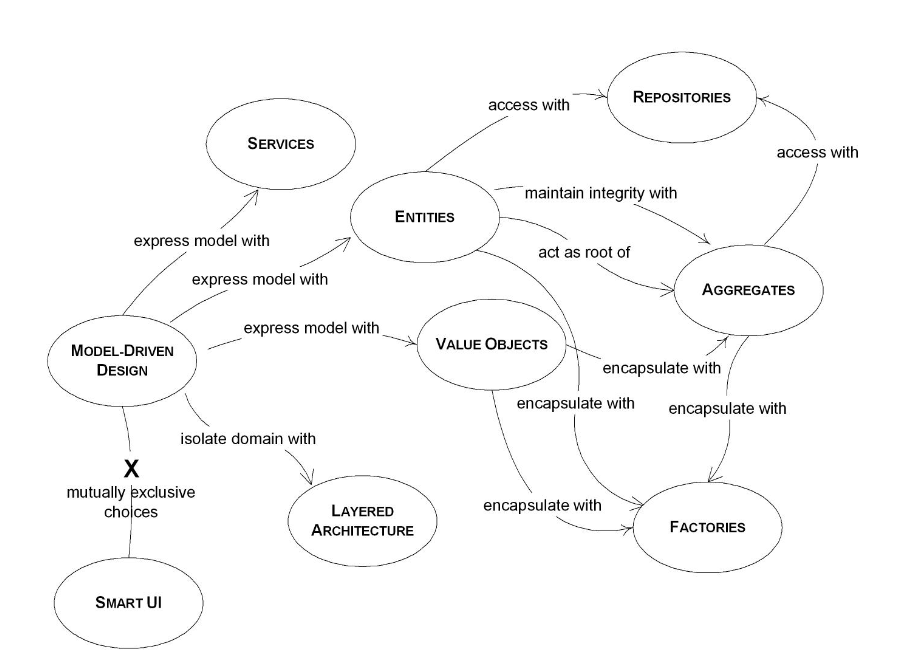
\includegraphics[scale = 0.8]{pictures/cac_mau_ky_thuat/temp.png}

\caption{vvn20206205}

\end{figure}

%!<! - - $ Vẽ lại sau: - - >

%!<! - - $ Vẽ lại sau: - - >

%!<! - - $ Vẽ lại sau: - - >

%!<! - - $ Vẽ lại sau: - - >

%!<! - - $ Vẽ lại sau: - - >

%!<! - - $ Vẽ lại sau: - - >

%!<! - - $ Vẽ lại sau: - - >

%!<! - - $ Vẽ lại sau: - - >

%!<! - - $ Vẽ lại sau: - - >

%!<! - - $ Vẽ lại sau: - - >

%!<! - - $ Vẽ lại sau: - - >

%!<! - - $ Vẽ lại sau: - - >

%!<! - - $ Vẽ lại sau: - - >

\section{Đối tượng miền (Domain Object)}

% Đối tượng miền (Domain Object)    được sử dụng để mô hình hóa    mô hình miền.  Đối tượng miền    được sử dụng để   triển khai   các quy tắc, các ràng buộc và các mối quan hệ   của nghiệp vụ.
Đối tượng miền   bao gồm:





\begin{itemize}
\item Đối tượng thực thể (Entities Objects)  
\item Đối tượng giá trị (Value Objects) 
\item  Miền dịch vụ (Service Domain) 

\end{itemize}

 
 
 

 

\subsection{Đối tượng thực thể (Entities Objects)}

% \subsection{Đối tượng thực thể (Entities Objects)}

%%%%%%%%%%%%%%%%%%%%%%%%%%%%%%%%%%

Định nghĩa:

% <!-- Một thực thể đại diện cho một đối tượng kinh doanh có thể nhận dạng duy nhất, bao gồm các thuộc tính và hành vi miền được xác định rõ ràng. -->

\begin{example}

\end{example}

% mối quan hệ giữa logic nghiệp vụ và các đối tượng thực thể.

% <!-- Một thực thể được xác định duy nhất trong một bối cảnh giới hạn. -->

% Các thực thể này và danh tính của chúng chỉ có ý nghĩa trong bối cảnh giới hạn tương ứng của chúng. Một thực thể có một tập hợp các thuộc tính được xác định bởi ngôn ngữ chung cho ngữ cảnh giới hạn .

% Một thực thể có một hành vi, nghĩa là nó đóng gói logic nghiệp vụ. Và logic kinh doanh này được thể hiện qua cách thức hoạt động.

% Khi các hoạt động này được thực hiện đối với thực thể, nó sẽ dẫn đến sự thay đổi trạng thái của thực thể.

Khi một số thao tác này được thực thi, chúng sẽ thay đổi trạng thái của tài khoản. Ví dụ: số dư có thể tăng hoặc giảm do thực hiện một số thao tác này.

13

00: 02: 23, 100--> 00: 02: 29, 160

Hãy xác định logic kinh doanh là gì, không phải kinh doanh. Logic đôi khi được gọi là logic miền.

14

00: 02: 29, 160--> 00: 02: 38, 680

Logic nghiệp vụ có thể bao gồm các quy tắc nghiệp vụ. Ví dụ: việc rút tiền sẽ không thành công nếu số dư nhỏ hơn số tiền rút.

15

00: 02: 38, 850--> 00: 02: 55, 860

Nó có thể là sự xác nhận. Ví dụ: số tiền rút không được nhỏ hơn hoặc bằng 0. Nó có thể là các phép tính, ví dụ, tính chéo thành phần cho tài khoản séc và nó có thể là các hoạt động có thể thay đổi trạng thái của thực thể.

16

00: 02: 55, 860--> 00: 03: 05, 880

Ví dụ: logic giao dịch rút tiền có thể được kết hợp để thực hiện tất cả những điều này được gọi là logic nghiệp vụ nói chung.

17

00: 03: 06, 330--> 00: 03: 15, 600

Hãy xem một ví dụ về logic nghiệp vụ hoặc hành vi. Trong trường hợp tài khoản séc, có thể có hoạt động rút tiền từ tài khoản.

18

00: 03: 15, 900--> 00: 03: 28, 320

Hoạt động rút tiền này có thể lấy số tiền rút làm đối số. Việc kiểm tra đầu tiên sẽ được thực hiện khi thực hiện thao tác rút tiền là kiểm tra số dư khả dụng.

19

00: 03: 28, 320--> 00: 03: 39, 840

Nếu số dư khả dụng nhỏ hơn số tiền rút thì giao dịch sẽ bị từ chối. Nếu không, giao dịch sẽ được chấp nhận và số dư sẽ bị giảm đi theo số tiền rút.

20

00: 03: 40, 140--> 00: 03: 49, 020

Đã đến lúc làm một bài kiểm tra nhanh. Hãy nhìn vào thực thể tài khoản kiểm tra này. Chúng ta có nghĩ rằng thực thể này bộc lộ một số logic kinh doanh không?

21

00: 03: 50, 700--> 00: 03: 58, 350

Câu trả lời là không, không phải vậy, và lý do tôi nói vậy là vì những thao tác này chỉ là getters và setters.

22

00: 03: 58, 350--> 00: 04: 08, 820

Tương tự, thao tác này là sở hữu đối tượng vào CSDL . Vì vậy, nhìn từ bề ngoài, có vẻ như thực thể này không bao gồm bất kỳ hoạt động kinh doanh nào.

23

00: 04: 08, 820--> 00: 04: 21, 180

Các thực thể logic chỉ có ý nghĩa trong bối cảnh ranh giới mà chúng được xác định. Người ta thường thấy các tên thực thể giống nhau xuất hiện trên nhiều ngữ cảnh được liên kết.

24

00: 04: 21, 630--> 00: 04: 29, 200

Nhưng chúng ta phải nhớ rằng định nghĩa của thực thể trong bối cảnh giới hạn này không được đảm bảo giữ nguyên.

25

00: 04: 29, 310--> 00: 04: 39, 300

Ví dụ: thực thể khách hàng trong tài khoản bán lẻ có thể trông không giống với thực thể khách hàng trong bối cảnh giới hạn thẻ tín dụng.

26

00: 04: 39, 660--> 00: 04: 53, 780

Hãy nhớ rằng các thực thể được xác định duy nhất trong một ngữ cảnh giới hạn, nhưng đôi khi có thể xảy ra trường hợp cùng một thuộc tính được sử dụng để xác định duy nhất thực thể trong các liên hệ công việc.

27

00: 04: 53, 790--> 00: 05: 05, 620

Nhưng đó hoàn toàn là sự trùng hợp ngẫu nhiên. Vì vậy, trong ví dụ này, số An sinh xã hội của khách hàng đang được sử dụng để nhận dạng duy nhất khách hàng trong cả hai địa chỉ liên hệ công việc này.

28

00: 05: 06, 180--> 00: 05: 26, 420

Hãy nhớ rằng, đó thực sự là sự trùng hợp ngẫu nhiên. Việc xác định các thực thể này của nhóm sẽ hoạt động độc lập với nhau và xác định các thuộc tính cũng như hoạt động cho các thực thể dựa trên yêu cầu trong từng bối cảnh nghiệp vụ, các thực thể được lưu trữ lâu dài.

29

00: 05: 26, 700--> 00: 05: 40, 000

Dữ liệu được lưu trữ dài hạn thể hiện trạng thái hiện tại của thực thể. Điều này phổ biến đối với RDBMS và không có CSDL đơn lẻ nào được sử dụng để lưu trữ liên tục các thực thể.

30

00: 05: 40, 620--> 00: 05: 56, 450

Trong trường hợp RDBMS, một bảng biểu thị một tập hợp các thực thể. Các quy tắc trong bảng biểu thị các thực thể được xác định duy nhất bằng cột khóa chính.

31

00: 05: 56, 700--> 00: 06: 06, 740

Các cột còn lại có các giá trị cho thuộc tính của từng thực thể. Đã đến lúc xem lại nhanh những điểm chính của bài giảng này.

32

00: 06: 06, 840--> 00: 06: 14, 640

Điều đầu tiên là các thực thể là các đối tượng kinh doanh chỉ có ý nghĩa trong một bối cảnh giới hạn.

33

00: 06: 14, 640--> 00: 06: 26, 760

Nơi chúng được xác định là các thực thể được xác định duy nhất trong bối cảnh giới hạn . Tiếp theo là định nghĩa của thực thể bao gồm thuộc tính và hành vi.

34

00: 06: 27, 060--> 00: 06: 35, 700

Hành vi này triển khai logic nghiệp vụ có thể thay đổi trạng thái của thực thể. Các thực thể được lưu trữ lâu dài.

%%%%%%%%%%%%%%%%%%%%%%%%%%%%%%%%%%

Đối tượng thực thể (Entities Objects) là đối tượng miền có có định danh riêng duy nhất. Định danh này được giữ nguyên xuyên suốt trạng thái hoạt động của hệ thống phần mềm.

Các thực thể là những đối tượng rất quan trọng của mô hình miền. Việc xác định xem một đối tượng có phải là thực thể hay không rất quan trọng.

Trong trường hợp CSDL quan hệ, một bảng biểu thị một tập hợp các thực thể. Các quy tắc trong bảng biểu thị các thực thể được xác định duy nhất bằng cột khóa chính.

Hành vi này triển khai logic nghiệp vụ có thể thay đổi trạng thái của thực thể. Các thực thể được lưu trữ lâu dài.

% %! Entity : https:// thiết kế hướng miền - practitioners.com/entity

% %! Entity : https:// thiết kế hướng miền - practitioners.com/entity

% %! Entity : https:// thiết kế hướng miền - practitioners.com/entity

% %! Entity : https:// thiết kế hướng miền - practitioners.com/entity

thực thể

Trong Thiết kế hướng miền (thiết kế hướng miền), thực thể là khái niệm cốt lõi đại diện cho một đối tượng miền có nhận dạng duy nhất. Thực thể là một đối tượng được phân biệt với các đối tượng khác dựa trên nhận dạng duy nhất của nó, thay vì thuộc tính hoặc giá trị của nó.

Các thực thể thường là các đối tượng quan trọng nhất trong mô hình miền và chúng thường có logic và hành vi nghiệp vụ phức tạp được liên kết với chúng. Họ cũng có thể có mối quan hệ với các thực thể, đối tượng giá trị hoặc dịch vụ miền khác.

Một thực thể có các đặc điểm sau:

Danh tính: Một thực thể có một danh tính duy nhất để phân biệt nó với các thực thể khác trong mô hình miền. Danh tính thường được biểu thị bằng ID hoặc khóa, chẳng hạn như ID khách hàng hoặc SKU sản phẩm.

Khả năng thay đổi: Các thuộc tính của thực thể có thể thay đổi theo thời gian trong khi vẫn duy trì được danh tính của nó. Ví dụ: tên hoặc địa chỉ của khách hàng có thể thay đổi nhưng ID khách hàng vẫn giữ nguyên.

Hành vi: Một thực thể có hành vi liên quan đến nó, thường là các quy tắc và logic nghiệp vụ phức tạp. Hành vi này thường được gói gọn trong chính thực thể đó.

Mối quan hệ: Một thực thể có thể có mối quan hệ với các thực thể, đối tượng giá trị hoặc dịch vụ miền khác. Ví dụ: khách hàng có thể có lịch sử đặt hàng hoặc giỏ hàng.

Các thực thể là một phần thiết yếu của mô hình miền và phải được thiết kế để thể hiện chính xác miền và các quy tắc kinh doanh của nó. Bằng cách lập mô hình chính xác các thực thể, nhà phát triển có thể tạo ra giải pháp phần mềm linh hoạt và dễ bảo trì hơn, đáp ứng nhu cầu của miền.

Một ví dụ

Hãy xem xét một nền tảng thương mại điện tử nơi khách hàng có thể đặt hàng sản phẩm. Trong mô hình miền này, Đơn hàng là một thực thể. Mỗi đơn hàng có một danh tính duy nhất và bất biến, chẳng hạn như số đơn hàng, giúp phân biệt nó với các đơn hàng khác trong hệ thống.

Thực thể Đơn hàng có thể có một số thuộc tính, chẳng hạn như thông tin khách hàng, chi tiết thanh toán và thông tin giao hàng. Nó cũng có thể có mối quan hệ với các thực thể khác, chẳng hạn như thực thể Sản phẩm và Khách hàng.

Hành vi của thực thể Đơn hàng bao gồm tạo và cập nhật đơn hàng, quản lý xử lý thanh toán và theo dõi trạng thái đơn hàng.

Dưới đây là ví dụ về giao diện của thực thể Đơn hàng trong mã:

public class Order {

private OrderId orderId;

private Customer customer;

private List<Product> products;

private Date orderDate;

private PaymentDetails paymentDetails;

private ShippingDetails shippingDetails;

public Order(OrderId orderId, Customer customer) {

this.orderId = orderId;

this.customer = customer;

this.products = Lists.newArrayList();

this.orderDate = LocalDate.now();

}

public void addProduct(Product product) {

products.add(product);

}

public void removeProduct(Product product) {

products.remove(product);

}

public void processPayment() {

// Process payment logic here...

}

public void shipOrder() {

// Shipping logic here...

}

// Other behavior methods here...

}

Trong ví dụ này, thực thể Đơn hàng có một ID duy nhất (orderId) xác định nó trong hệ thống, cùng với các thuộc tính khác như customer, < /span>, gói gọn logic kinh doanh được liên kết với thực thể đơn hàng., và,, . Thực thể cũng có các phương thức hành vi, chẳng hạn như và, products, orderDatepaymentDetailsshippingDetailsaddProductremoveProductprocessPaymentshipOrder

% %! Entity : https:// thiết kế hướng miền - practitioners.com/entity

% %! Entity : https:// thiết kế hướng miền - practitioners.com/entity

% %! Entity : https:// thiết kế hướng miền - practitioners.com/entity

% %! Entity Identity : https:// thiết kế hướng miền - practitioners.com/entity - identity

% %! Entity Identity : https:// thiết kế hướng miền - practitioners.com/entity - identity

% %! Entity Identity : https:// thiết kế hướng miền - practitioners.com/entity - identity

% %! Entity Identity : https:// thiết kế hướng miền - practitioners.com/entity - identity

Trang chủTrang chủBảng chú giảiNhận dạng thực thể

Nhận dạng thực thể

Danh tính của một thực thể phải là duy nhất và bất biến, nghĩa là nó không được thay đổi trong suốt vòng đời của thực thể đó. Việc thay đổi danh tính của một thực thể có thể gây ra hậu quả nghiêm trọng, chẳng hạn như gây ra sự không nhất quán về dữ liệu hoặc phá vỡ mối quan hệ với các thực thể hoặc đối tượng giá trị khác. Ví dụ: nếu ID của khách hàng bị thay đổi, điều đó có thể dẫn đến nhầm lẫn khi theo dõi lịch sử mua hàng của họ hoặc các tương tác khác với hệ thống.

Điều quan trọng cần lưu ý là các thuộc tính của thực thể, chẳng hạn như tên hoặc địa chỉ, có thể thay đổi mà không ảnh hưởng đến danh tính của thực thể đó. Những thay đổi này phải được quản lý thông qua việc đóng gói thích hợp hành vi và logic kinh doanh của thực thể.

Tóm lại, danh tính của một thực thể phải là duy nhất và bất biến, đồng thời những thay đổi đối với các thuộc tính của thực thể sẽ không ảnh hưởng đến danh tính của thực thể đó. Bằng cách tuân thủ nguyên tắc này, các nhà phát triển có thể tạo ra một mô hình miền nhất quán và dễ bảo trì hơn, thể hiện chính xác miền kinh doanh.

Làm thế nào để chọn một danh tính thực thể tốt

Chọn danh tính phù hợp cho một thực thể là một phần quan trọng trong việc thiết kế mô hình miền trong Thiết kế hướng miền (thiết kế hướng miền). Dưới đây là một số phương pháp hay để chọn danh tính của một thực thể:

Chọn một danh tính duy nhất: Danh tính của một thực thể phải là duy nhất trong mô hình miền và nó không được thay đổi trong suốt vòng đời của thực thể. Danh tính của một thực thể phải được xác định theo yêu cầu kinh doanh, chẳng hạn như mã định danh duy nhất như số sê - ri, ID khách hàng hoặc số an sinh xã hội.

Chọn danh tính ổn định: Danh tính của thực thể phải ổn định, nghĩa là danh tính không được thay đổi theo thời gian. Danh tính ổn định cho phép tính nhất quán và độ chính xác trong mô hình miền và nó có thể ngăn ngừa lỗi trong hệ thống. Ví dụ: nếu ID của khách hàng thay đổi, việc theo dõi lịch sử mua hàng của họ hoặc các tương tác khác với hệ thống có thể gây nhầm lẫn.

Chọn danh tính dễ nhận dạng: Danh tính của thực thể phải dễ nhận dạng, tốt nhất là bởi người đọc. Ví dụ: việc sử dụng UUID hoặc GUID có thể không dễ nhận biết như tên hoặc số ID của khách hàng.

Chọn một danh tính có thể được sử dụng nhất quán trong toàn bộ mô hình miền: Danh tính của một thực thể phải nhất quán trong toàn bộ mô hình miền và nó phải được sử dụng nhất quán trong mọi ngữ cảnh mà thực thể đó được tham chiếu.

Xem xét khả năng mở rộng và hiệu suất: Việc chọn một danh tính có thể mở rộng quy mô và hoạt động tốt cũng rất quan trọng, đặc biệt đối với các hệ thống có khối lượng dữ liệu lớn hoặc thông lượng cao.

Bằng cách làm theo những thực tiễn này, nhà phát triển có thể chọn danh tính phù hợp cho các thực thể thể hiện chính xác mô hình miền và cung cấp giải pháp phần mềm linh hoạt và có thể bảo trì.

% %! Entity Identity : https:// thiết kế hướng miền - practitioners.com/entity - identity

% %! Entity Identity : https:// thiết kế hướng miền - practitioners.com/entity - identity

% %! Entity Identity : https:// thiết kế hướng miền - practitioners.com/entity - identity

% %! Entity Identity : https:// thiết kế hướng miền - practitioners.com/entity - identity



\subsection{Đối tượng giá trị (Value Objects)}

% Đối tượng miền hoặc đối tượng giá trị, là đối tượng đại diện cho một đặc điểm của miền mà không có nhận dạng riêng.

% % Một đối tượng được dùng để mô tả các khía cạnh cố định của một miền và không có định danh.

% Đối tượng giá trị không có danh tính duy nhất.

% Đối tượng giá trị được tạo trong bộ nhớ tiến trình và sau đó bị hủy sau khi nó đã phục vụ mục đích của nó.

% Một điểm khác biệt quan trọng giữa các thực thể và đối tượng giá trị là đối tượng giá trị không tồn tại lâu dài trong CSDL.

% %! VD

% %! chúng ta sẽ đặt logic xác thực cho địa chỉ email ở đâu?

% %! xác nhận kỹ thuật không liên quan đến bất kỳ khái niệm kinh doanh nào.

% %! tạo một đối tượng giá trị để xác thực địa chỉ email.

% %! Kết quả là, thực thể khách hàng sẽ sạch hơn và đơn giản hơn nhiều trong việc thực hiện.

% %! % Value Object -

% %! Value Object : https:// thiết kế hướng miền - practitioners.com/home/glossary/value - object

% %! Value Object : https:// thiết kế hướng miền - practitioners.com/home/glossary/value - object

% %! Value Object : https:// thiết kế hướng miền - practitioners.com/home/glossary/value - object

% %! [[Value Object]] An object that describes some characteristic or attribute but carries no concept of identity.

Trang chủTrang chủBảng chú giảiĐối tượng giá trị

Đối tượng giá trị

Trong Thiết kế hướng miền (thiết kế hướng miền), đối tượng giá trị là một đối tượng đại diện cho một khái niệm hoặc ý tưởng trong mô hình miền không có danh tính duy nhất hoặc tuổi thọ vượt quá tuổi thọ của thực thể chứa đối tượng.

Một đối tượng giá trị được xác định bởi các thuộc tính của nó và nó không thể thay đổi, nghĩa là trạng thái của nó không thể thay đổi sau khi được tạo. Các đối tượng giá trị thường được sử dụng để biểu thị số lượng, phép đo, ngày tháng, tiền tệ hoặc các khái niệm khác có thể được biểu thị dưới dạng kết hợp các thuộc tính.

Vì các đối tượng giá trị không có danh tính duy nhất nên chúng có thể được sao chép và chia sẻ tự do mà không ảnh hưởng đến tính nhất quán của mô hình miền. Các đối tượng giá trị cũng được so sánh dựa trên thuộc tính của chúng chứ không phải danh tính của chúng, điều này cho phép so sánh linh hoạt và trực quan hơn.

Trong triển khai phần mềm, các đối tượng giá trị thường được tạo dưới dạng các lớp bất biến, không có danh tính riêng và chúng thường được triển khai như một phần của thực thể hoặc tập hợp chứa. Bằng cách sử dụng các đối tượng giá trị trong mô hình miền, nhà phát triển có thể tạo mã có tính biểu cảm hơn, dễ bảo trì và mở rộng hơn để phản ánh tốt hơn miền kinh doanh.

Một ví dụ

Giả sử chúng ta đang xây dựng một trang web thương mại điện tử và chúng ta có yêu cầu thể hiện giá trong mô hình miền. Giá là một ứng cử viên phù hợp cho đối tượng giá trị vì nó có thể được biểu diễn dưới dạng kết hợp các thuộc tính (ví dụ: tiền tệ và số lượng) và không có đặc điểm nhận dạng duy nhất của riêng nó.

Đây là một ví dụ cực kỳ đơn giản về đối tượng Giá trị giá trong Java:

1

2

3

4

5

6

7

số 8

9

10

11

12

13

14

15

16

17

18

19

class Price {

private final Currency currency;

private final BigDecimal amount;

public Price(Currency currency, BigDecimal amount) {

this.currency = currency;

this.amount = amount;

}

public Currency getCurrency() {

return currency;

}

public BigDecimal getAmount() {

return amount;

}

// Other methods and business logic specific to the Price concept

}

Trong ví dụ này, đối tượng giá trị Price có hai thuộc tính: currency và amount. Thuộc tính currency đại diện cho đơn vị tiền tệ của giá (ví dụ: USD, EUR, v.v.), trong khi thuộc tính amount đại diện cho giá trị bằng số của giá. Đối tượng Price là bất biến và trạng thái của nó không thể thay đổi sau khi được tạo. Đối tượng Price cũng xác định các phương thức để truy xuất các thuộc tính của nó (ví dụ: getCurrency() và getAmount()), cũng như các phương thức khác dành riêng cho < khái niệm /span>). hoặc Price (ví dụ: phương thức add()subtract()

Bằng cách sử dụng đối tượng giá trị Price, chúng tôi có thể đảm bảo rằng giá được thể hiện nhất quán trong toàn bộ mô hình miền và chúng tôi có thể thực hiện các so sánh và tính toán linh hoạt và trực quan hơn về giá.

Đối tượng giá trị so với thực thể

Đối tượng giá trị trong một giải pháp có thể trở thành một thực thể trong giải pháp khác. Sự khác biệt giữa các đối tượng giá trị và các thực thể phụ thuộc vào ngữ cảnh và dựa trên nhu cầu của mô hình miền.

Trong một ngữ cảnh, một đối tượng có thể được coi là một đối tượng giá trị vì nó được xác định bởi các thuộc tính của nó và không có một danh tính duy nhất. Tuy nhiên, trong một bối cảnh khác hoặc một giải pháp khác, cùng một đối tượng có thể được coi là một thực thể vì nó có một danh tính duy nhất và có thể được lưu giữ trong CSDL hoặc có tuổi thọ vượt quá đối tượng chứa.

Ví dụ: hãy xem xét một đối tượng Person trong miền nhân sự. Trong một ngữ cảnh, đối tượng Person có thể được coi là một đối tượng giá trị vì nó được xác định bởi các thuộc tính của nó, chẳng hạn như tên, ngày sinh và số an sinh xã hội. Tuy nhiên, trong một ngữ cảnh khác hoặc một giải pháp khác, đối tượng Person có thể được coi là một thực thể vì nó có một danh tính duy nhất và có thể được duy trì trong CSDL hoặc được sử dụng trên các ngữ cảnh giới hạn khác nhau.

Cuối cùng, việc lựa chọn mô hình hóa một đối tượng là đối tượng giá trị hay thực thể phụ thuộc vào nhu cầu của mô hình miền và các yêu cầu cụ thể của giải pháp phần mềm đang được phát triển. Điều quan trọng là chọn các khái niệm mô hình phù hợp để thể hiện chính xác miền và cung cấp giải pháp phần mềm linh hoạt và có thể bảo trì.

% %! Value Object : https:// thiết kế hướng miền - practitioners.com/home/glossary/value - object

% %! Value Object : https:// thiết kế hướng miền - practitioners.com/home/glossary/value - object

% %! Value Object : https:// thiết kế hướng miền - practitioners.com/home/glossary/value - object



\subsection{Miền dịch vụ (Service Domain)}

% % %! Service : https:// thiết kế hướng miền - practitioners.com/ dịch vụ

% %! Service : https:// thiết kế hướng miền - practitioners.com/ dịch vụ

% %! Service : https:// thiết kế hướng miền - practitioners.com/ dịch vụ

% %! Service : https:// thiết kế hướng miền - practitioners.com/ dịch vụ

% %! Service : https:// thiết kế hướng miền - practitioners.com/ dịch vụ

% %! [[Service]] An operation offered as an interface that stands alone in the model, with no encapsulated state.

Chuyển đến nội dung

Đối với người hành nghề bởi người hành nghề

Tìm kiếm

Thiết kế hướng miền: Hướng dẫn dành cho người thực hành

Câu hỏi thường gặp

Bảng chú giải

Về chúng tôi

Cuốn sách của chúng tôi!

Trang chủTrang chủBảng chú giảiDịch vụ

Dịch vụ

Trong thiết kế hướng miền, dịch vụ là một phần của lớp miền triển khai logic miền hoặc trường hợp sử dụng không phù hợp một cách tự nhiên với một thực thể hoặc đối tượng giá trị cụ thể. Nó thường điều phối các tương tác giữa nhiều thực thể hoặc tập hợp. Một dịch vụ đại diện cho một hoạt động gắn kết và không trạng thái có đầu vào và đầu ra. Nó không có trạng thái bền vững và không cần phải khởi tạo. Các dịch vụ thường có tên phản ánh mục đích miền của chúng, chẳng hạn như `OrderProcessingService` hoặc `PaymentService`.

Có một số trường hợp nhất định mà việc sử dụng dịch vụ có thể không phù hợp.

Thứ nhất, nếu logic nghiệp vụ có thể được liên kết với một thực thể hoặc đối tượng giá trị, có thể tốt hơn nếu gói gọn logic trong thực thể hoặc đối tượng giá trị đó. Điều này có thể giúp cải thiện tính gắn kết của mã và làm cho mã dễ hiểu hơn.

Thứ hai, nếu logic nghiệp vụ liên quan đến nhiều thực thể hoặc tập hợp được liên kết chặt chẽ với nhau thì tốt hơn là chúng ta nên đánh giá lại thiết kế của bản thân các uẩn. Trong những trường hợp như vậy, có thể phù hợp hơn nếu phân chia các tập hợp hoặc xác định lại ranh giới của chúng để giảm sự ghép nối và cải thiện khả năng bảo trì.

Cuối cùng, nếu logic nghiệp vụ liên quan đến các hệ thống hoặc cơ sở hạ tầng bên ngoài thì tốt hơn nên sử dụng lớp chống đổ vỡ hoặc mẫu bộ chuyển đổi để tách biệt mô hình miền khỏi các phụ thuộc bên ngoài. Điều này có thể giúp giảm khả năng ghép nối và cải thiện tính linh hoạt của hệ thống.

Ví dụ

Dưới đây là ví dụ về một dịch vụ trong Java có liên quan đến nhiều hơn một tổng hợp:

1

2

3

4

5

6

7

số 8

9

10

11

12

13

14

15

public class OrderService {

private final OrderRepository orderRepository;

private final ProductRepository productRepository;

public void createOrder(Order order) {

for (OrderItem item: order.getItems()) {

Product product = productRepository.findById(item.getProductId());

product.reduceStockBy(item.getQuantity());

productRepository.save(product);

}

orderRepository.save(order);

}

// Other methods...

}

Trong ví dụ này, OrderService chịu trách nhiệm tạo đơn đặt hàng và nó tương tác với hai tập hợp: Order và Product. Tổng hợp Order đại diện cho đơn đặt hàng do khách hàng đặt, trong khi tổng hợp Product đại diện cho một sản phẩm có thể được đặt hàng.

Phương thức createOrder cập nhật kho của từng sản phẩm trong đơn hàng bằng cách gọi phương thức save trên ProductRepository, và sau đó tự lưu đơn hàng bằng cách gọi phương thức save trên OrderRepository.

Thể loại

Phân tích

điều cơ bản

thiết kế hướng miền

thiết kế

câu hỏi thường gặp

Khả năng lãnh đạo

hoa văn

Blog tại WordPress.com.

% %! Service : https:// thiết kế hướng miền - practitioners.com/ dịch vụ

% %! Service : https:// thiết kế hướng miền - practitioners.com/ dịch vụ

% %! Service : https:// thiết kế hướng miền - practitioners.com/ dịch vụ

% %! Service : https:// thiết kế hướng miền - practitioners.com/ dịch vụ

% %! Service : https:// thiết kế hướng miền - practitioners.com/ dịch vụ

% %! Service : https:// thiết kế hướng miền - practitioners.com/ dịch vụ



%! Hướng dẫn 7/4

%! Hướng dẫn 7/5

% \subsubsection{xxxxxxx}

% 
\begin{titlepage}

% Vẽ hình chữ nhật

\begin{tikzpicture}[remember picture, overlay]\draw [line width = 3pt]($ (current page.north west) + (3.0cm, - 2.5cm)$)rectangle($ (current page.south east) + (- 2.5cm, 2.5cm)$);\draw [line width = 0.5pt]($ (current page.north west) + (3.1cm, - 2.6cm)$)rectangle($ (current page.south east) + (- 2.6cm, 2.6cm)$);\end{tikzpicture}

\begin{center}

\vspace{- 0.4cm}

\textbf{ĐẠI HỌC BÁCH KHOA HÀ NỘI} \\

\textbf{VIỆN TOÁN ỨNG DỤNG VÀ TIN HỌC} \\

\textbf{******}

\vspace{0.8cm}

\begin{figure}[H]

\centering


\includegraphics[scale = 0.5]{pictures/hust/main.png}

\end{figure}

\vspace{0.7cm}

\textbf{\fontsize{16pt}{30pt}\selectfont {BÁO CÁO ĐỒ ÁN II}}

\vspace{1cm}

\textbf{\fontsize{16pt}{30pt}\selectfont {ĐỀ TÀI:}} \\

\textbf{\fontsize{20pt}{24pt}\selectfont {Sử dụng thiết kế hướng miền \\ xây dựng kiến trúc vi dịch vụ cho \\ bài toán hóa đơn điện tử}} \\

\end{center}

\vspace{0.3cm}

\begin{center}

\textbf{\fontsize{10pt}{24pt}\selectfont {Chuyên ngành: Toán Tin}}

\end{center}

\vspace{0.7cm}

\hspace{3cm}\begin{minipage}{0.7\textwidth}

\begin{tabular}{l l l}

\textbf{\fontsize{10pt}{24pt}\selectfont {Giảng viên hướng dẫn}} & \textbf{\fontsize{10pt}{24pt}\selectfont {TS. Vũ Thành Nam}} \\

\textbf{\fontsize{10pt}{24pt}\selectfont {Sinh viên thực hiện}} & \textbf{\fontsize{10pt}{24pt}\selectfont {Vũ Văn Nghĩa}} \\

\textbf{\fontsize{10pt}{24pt}\selectfont {Mã số sinh viên}} & \textbf{\fontsize{10pt}{24pt}\selectfont {20206205}} \\

\textbf{\fontsize{10pt}{24pt}\selectfont {Lớp}} & \textbf{\fontsize{10pt}{24pt}\selectfont {Toán Tin 02 - K65}} \\

\end{tabular}

\end{minipage}

\vfill

\begin{center}

\textbf{Hà Nội, \the\year}

% \textbf{Hà Nội, \the\month~/~\the\year}

% \textbf{Hà Nội, \the\month~-~\the\year}

\end{center}

\end{titlepage}



\begin{titlepage}

% Vẽ hình chữ nhật

\begin{tikzpicture}[remember picture, overlay]\draw [line width = 3pt]($ (current page.north west) + (3.0cm, - 2.5cm)$)rectangle($ (current page.south east) + (- 2.5cm, 2.5cm)$);\draw [line width = 0.5pt]($ (current page.north west) + (3.1cm, - 2.6cm)$)rectangle($ (current page.south east) + (- 2.6cm, 2.6cm)$);\end{tikzpicture}

\begin{center}

\vspace{- 0.4cm}

\textbf{ĐẠI HỌC BÁCH KHOA HÀ NỘI} \\

\textbf{VIỆN TOÁN ỨNG DỤNG VÀ TIN HỌC} \\

\textbf{******}

\vspace{0.8cm}

\begin{figure}[H]

\centering


\includegraphics[scale = 0.5]{pictures/hust/main.png}

\end{figure}

\vspace{0.7cm}

\textbf{\fontsize{16pt}{30pt}\selectfont {BÁO CÁO ĐỒ ÁN II}}

\vspace{1cm}

\textbf{\fontsize{16pt}{30pt}\selectfont {ĐỀ TÀI:}} \\

\textbf{\fontsize{20pt}{24pt}\selectfont {Sử dụng thiết kế hướng miền \\ xây dựng kiến trúc vi dịch vụ cho \\ bài toán hóa đơn điện tử}} \\

\end{center}

\vspace{0.3cm}

\begin{center}

\textbf{\fontsize{10pt}{24pt}\selectfont {Chuyên ngành: Toán Tin}}

\end{center}

\vspace{0.7cm}

\hspace{3cm}\begin{minipage}{0.7\textwidth}

\begin{tabular}{l l l}

\textbf{\fontsize{10pt}{24pt}\selectfont {Giảng viên hướng dẫn}} & \textbf{\fontsize{10pt}{24pt}\selectfont {TS. Vũ Thành Nam}} \\

\textbf{\fontsize{10pt}{24pt}\selectfont {Sinh viên thực hiện}} & \textbf{\fontsize{10pt}{24pt}\selectfont {Vũ Văn Nghĩa}} \\

\textbf{\fontsize{10pt}{24pt}\selectfont {Mã số sinh viên}} & \textbf{\fontsize{10pt}{24pt}\selectfont {20206205}} \\

\textbf{\fontsize{10pt}{24pt}\selectfont {Lớp}} & \textbf{\fontsize{10pt}{24pt}\selectfont {Toán Tin 02 - K65}} \\

\end{tabular}

\end{minipage}

\vfill

\begin{center}

\textbf{Hà Nội, \the\year}

% \textbf{Hà Nội, \the\month~/~\the\year}

% \textbf{Hà Nội, \the\month~-~\the\year}

\end{center}

\end{titlepage}



\begin{center}

{\bfseries NHẬN XÉT CỦA GIẢNG VIÊN HƯỚNG DẪN}

\end{center}

\begin{enumerate}

\item Mục đích và nội dung của đồ án:

\vspace{20ex}

\item Kết quả đạt được:

\vspace{20ex}

\item Ý thức làm việc của sinh viên:

\vspace{20ex}

\end{enumerate}

\hspace{0.4\textwidth}\begin{minipage}{0.5\textwidth}

\noindent\begin{center}

\textit{Hà Nội, \today} \\

\textbf{Giảng viên hướng dẫn} \\

\textit{(Ký và ghi rõ họ tên)}

\vspace{2cm}

\textbf{TS. Vũ Thành Nam}

\end{center}

\end{minipage}

\pagestyle{empty}



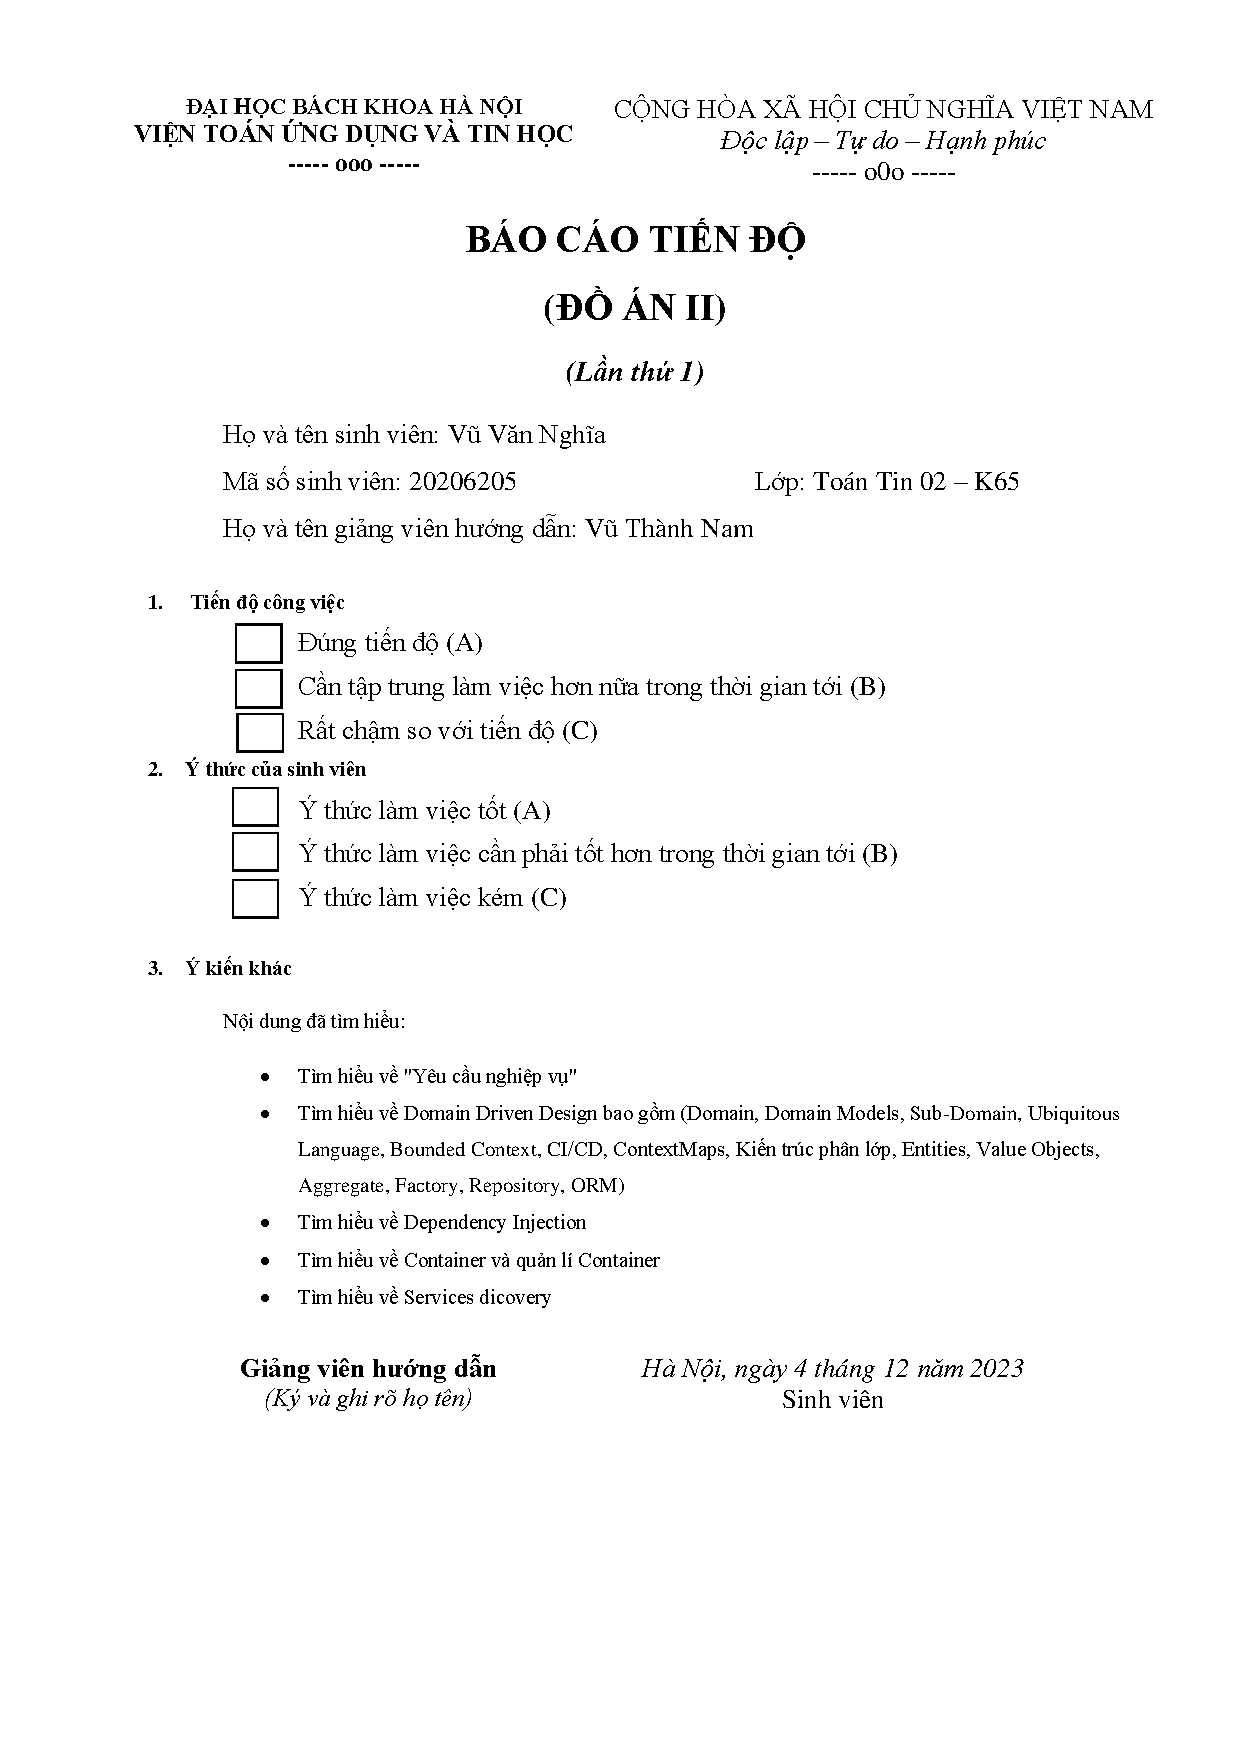
\includepdf[pages = -]{contents/bao_cao_tien_do_1.pdf}

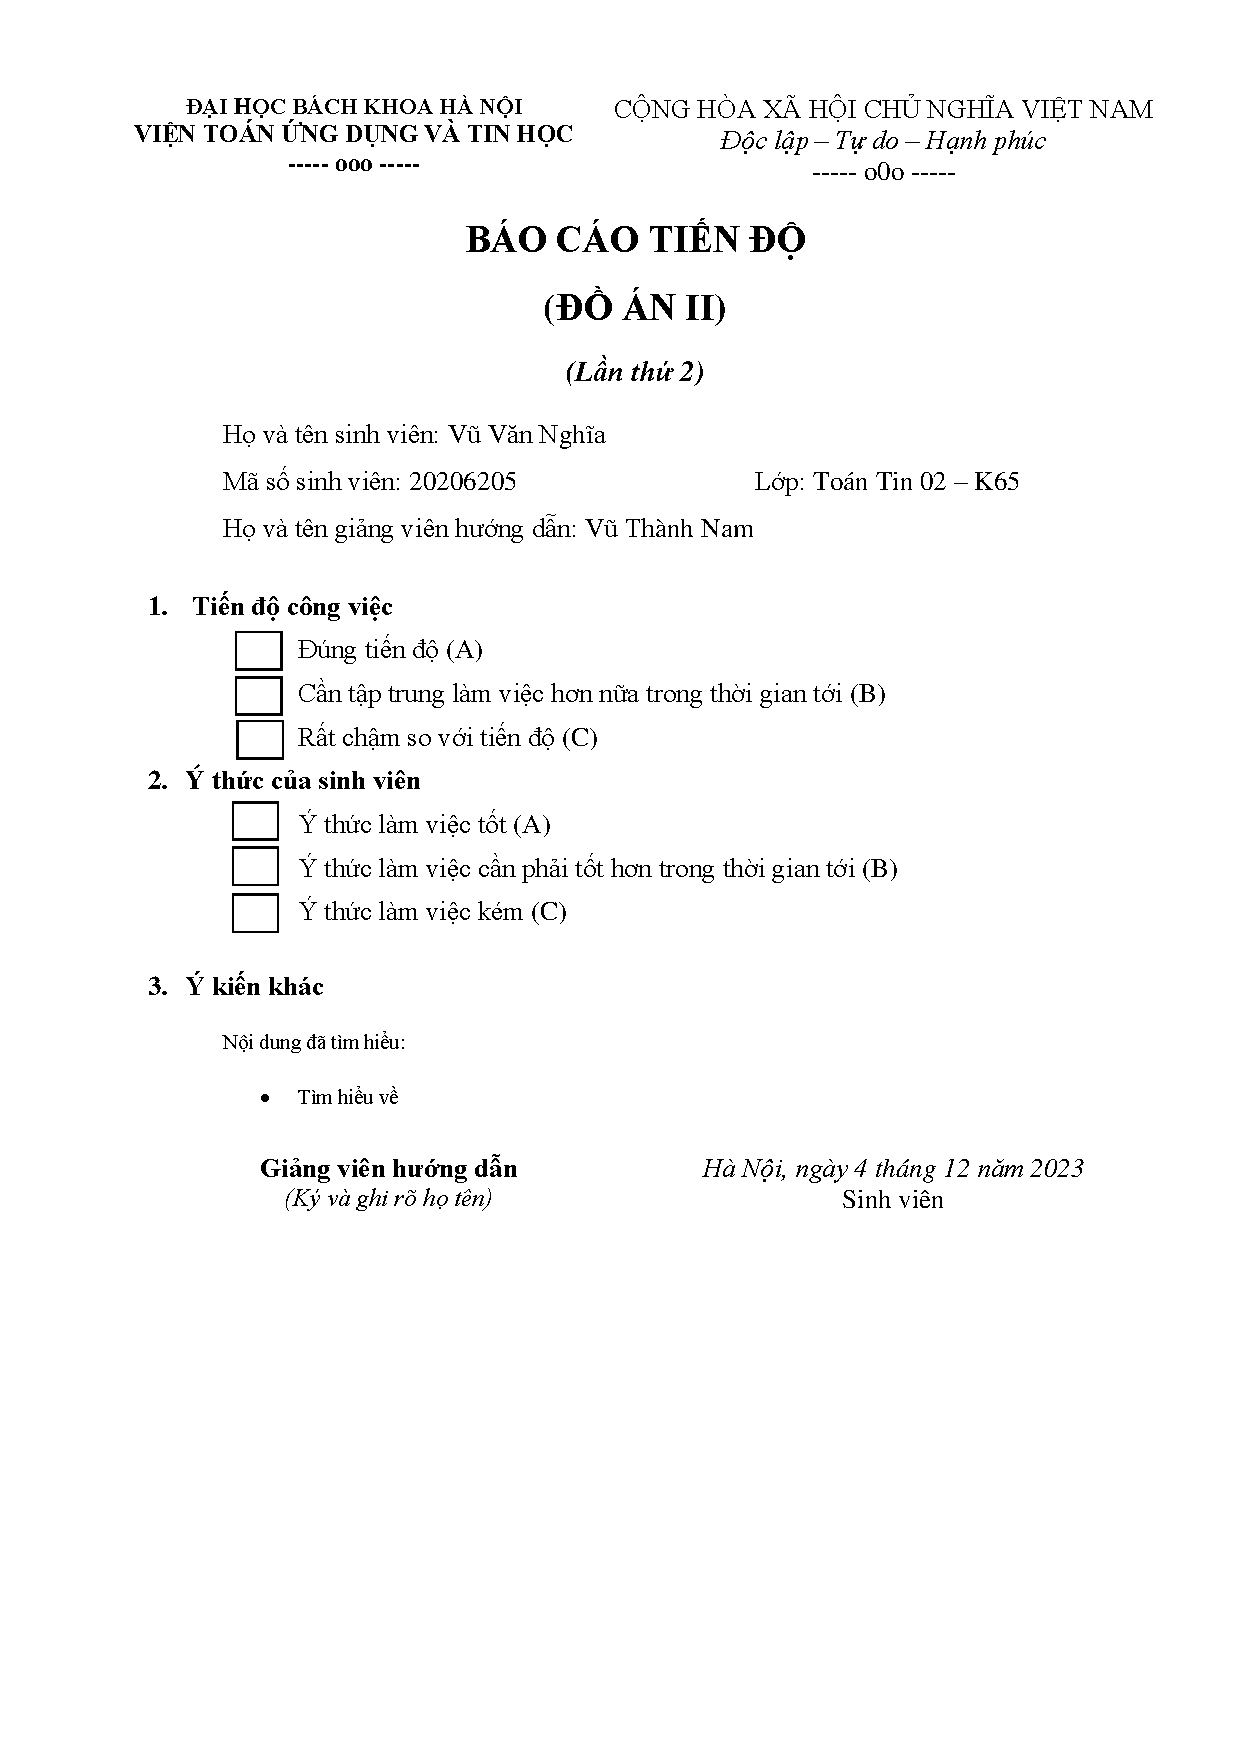
\includepdf[pages = -]{contents/bao_cao_tien_do_2.pdf}

%%%%%%%%%%%%%%%%%%%%%%%%%%%%%%%%%%

\end{document} % Kết thúc

% kết luận, tài liệu tham khảo

% \bibliographystyle{plain}

% \bibliography{references}

%%%%%%%%%%%%%%%%%%%%%%%%%%%%%%%%%%

% % %! Aggregates/ /

% % Tổng hợp là đối tượng kinh doanh trung tâm trong Bối cảnh bị giới hạn của chúng ta và xác định phạm vi nhất quán trong bối cảnh bị giới hạn đó.

% % Tổng hợp = Mã định danh chính của Bối cảnh bị giới hạn của chúng ta

% \subsubsection{xxxxxxx}

% % 
\begin{titlepage}

% Vẽ hình chữ nhật

\begin{tikzpicture}[remember picture, overlay]\draw [line width = 3pt]($ (current page.north west) + (3.0cm, - 2.5cm)$)rectangle($ (current page.south east) + (- 2.5cm, 2.5cm)$);\draw [line width = 0.5pt]($ (current page.north west) + (3.1cm, - 2.6cm)$)rectangle($ (current page.south east) + (- 2.6cm, 2.6cm)$);\end{tikzpicture}

\begin{center}

\vspace{- 0.4cm}

\textbf{ĐẠI HỌC BÁCH KHOA HÀ NỘI} \\

\textbf{VIỆN TOÁN ỨNG DỤNG VÀ TIN HỌC} \\

\textbf{******}

\vspace{0.8cm}

\begin{figure}[H]

\centering


\includegraphics[scale = 0.5]{pictures/hust/main.png}

\end{figure}

\vspace{0.7cm}

\textbf{\fontsize{16pt}{30pt}\selectfont {BÁO CÁO ĐỒ ÁN II}}

\vspace{1cm}

\textbf{\fontsize{16pt}{30pt}\selectfont {ĐỀ TÀI:}} \\

\textbf{\fontsize{20pt}{24pt}\selectfont {Sử dụng thiết kế hướng miền \\ xây dựng kiến trúc vi dịch vụ cho \\ bài toán hóa đơn điện tử}} \\

\end{center}

\vspace{0.3cm}

\begin{center}

\textbf{\fontsize{10pt}{24pt}\selectfont {Chuyên ngành: Toán Tin}}

\end{center}

\vspace{0.7cm}

\hspace{3cm}\begin{minipage}{0.7\textwidth}

\begin{tabular}{l l l}

\textbf{\fontsize{10pt}{24pt}\selectfont {Giảng viên hướng dẫn}} & \textbf{\fontsize{10pt}{24pt}\selectfont {TS. Vũ Thành Nam}} \\

\textbf{\fontsize{10pt}{24pt}\selectfont {Sinh viên thực hiện}} & \textbf{\fontsize{10pt}{24pt}\selectfont {Vũ Văn Nghĩa}} \\

\textbf{\fontsize{10pt}{24pt}\selectfont {Mã số sinh viên}} & \textbf{\fontsize{10pt}{24pt}\selectfont {20206205}} \\

\textbf{\fontsize{10pt}{24pt}\selectfont {Lớp}} & \textbf{\fontsize{10pt}{24pt}\selectfont {Toán Tin 02 - K65}} \\

\end{tabular}

\end{minipage}

\vfill

\begin{center}

\textbf{Hà Nội, \the\year}

% \textbf{Hà Nội, \the\month~/~\the\year}

% \textbf{Hà Nội, \the\month~-~\the\year}

\end{center}

\end{titlepage}



\begin{titlepage}

% Vẽ hình chữ nhật

\begin{tikzpicture}[remember picture, overlay]\draw [line width = 3pt]($ (current page.north west) + (3.0cm, - 2.5cm)$)rectangle($ (current page.south east) + (- 2.5cm, 2.5cm)$);\draw [line width = 0.5pt]($ (current page.north west) + (3.1cm, - 2.6cm)$)rectangle($ (current page.south east) + (- 2.6cm, 2.6cm)$);\end{tikzpicture}

\begin{center}

\vspace{- 0.4cm}

\textbf{ĐẠI HỌC BÁCH KHOA HÀ NỘI} \\

\textbf{VIỆN TOÁN ỨNG DỤNG VÀ TIN HỌC} \\

\textbf{******}

\vspace{0.8cm}

\begin{figure}[H]

\centering


\includegraphics[scale = 0.5]{pictures/hust/main.png}

\end{figure}

\vspace{0.7cm}

\textbf{\fontsize{16pt}{30pt}\selectfont {BÁO CÁO ĐỒ ÁN II}}

\vspace{1cm}

\textbf{\fontsize{16pt}{30pt}\selectfont {ĐỀ TÀI:}} \\

\textbf{\fontsize{20pt}{24pt}\selectfont {Sử dụng thiết kế hướng miền \\ xây dựng kiến trúc vi dịch vụ cho \\ bài toán hóa đơn điện tử}} \\

\end{center}

\vspace{0.3cm}

\begin{center}

\textbf{\fontsize{10pt}{24pt}\selectfont {Chuyên ngành: Toán Tin}}

\end{center}

\vspace{0.7cm}

\hspace{3cm}\begin{minipage}{0.7\textwidth}

\begin{tabular}{l l l}

\textbf{\fontsize{10pt}{24pt}\selectfont {Giảng viên hướng dẫn}} & \textbf{\fontsize{10pt}{24pt}\selectfont {TS. Vũ Thành Nam}} \\

\textbf{\fontsize{10pt}{24pt}\selectfont {Sinh viên thực hiện}} & \textbf{\fontsize{10pt}{24pt}\selectfont {Vũ Văn Nghĩa}} \\

\textbf{\fontsize{10pt}{24pt}\selectfont {Mã số sinh viên}} & \textbf{\fontsize{10pt}{24pt}\selectfont {20206205}} \\

\textbf{\fontsize{10pt}{24pt}\selectfont {Lớp}} & \textbf{\fontsize{10pt}{24pt}\selectfont {Toán Tin 02 - K65}} \\

\end{tabular}

\end{minipage}

\vfill

\begin{center}

\textbf{Hà Nội, \the\year}

% \textbf{Hà Nội, \the\month~/~\the\year}

% \textbf{Hà Nội, \the\month~-~\the\year}

\end{center}

\end{titlepage}



\begin{center}

{\bfseries NHẬN XÉT CỦA GIẢNG VIÊN HƯỚNG DẪN}

\end{center}

\begin{enumerate}

\item Mục đích và nội dung của đồ án:

\vspace{20ex}

\item Kết quả đạt được:

\vspace{20ex}

\item Ý thức làm việc của sinh viên:

\vspace{20ex}

\end{enumerate}

\hspace{0.4\textwidth}\begin{minipage}{0.5\textwidth}

\noindent\begin{center}

\textit{Hà Nội, \today} \\

\textbf{Giảng viên hướng dẫn} \\

\textit{(Ký và ghi rõ họ tên)}

\vspace{2cm}

\textbf{TS. Vũ Thành Nam}

\end{center}

\end{minipage}

\pagestyle{empty}



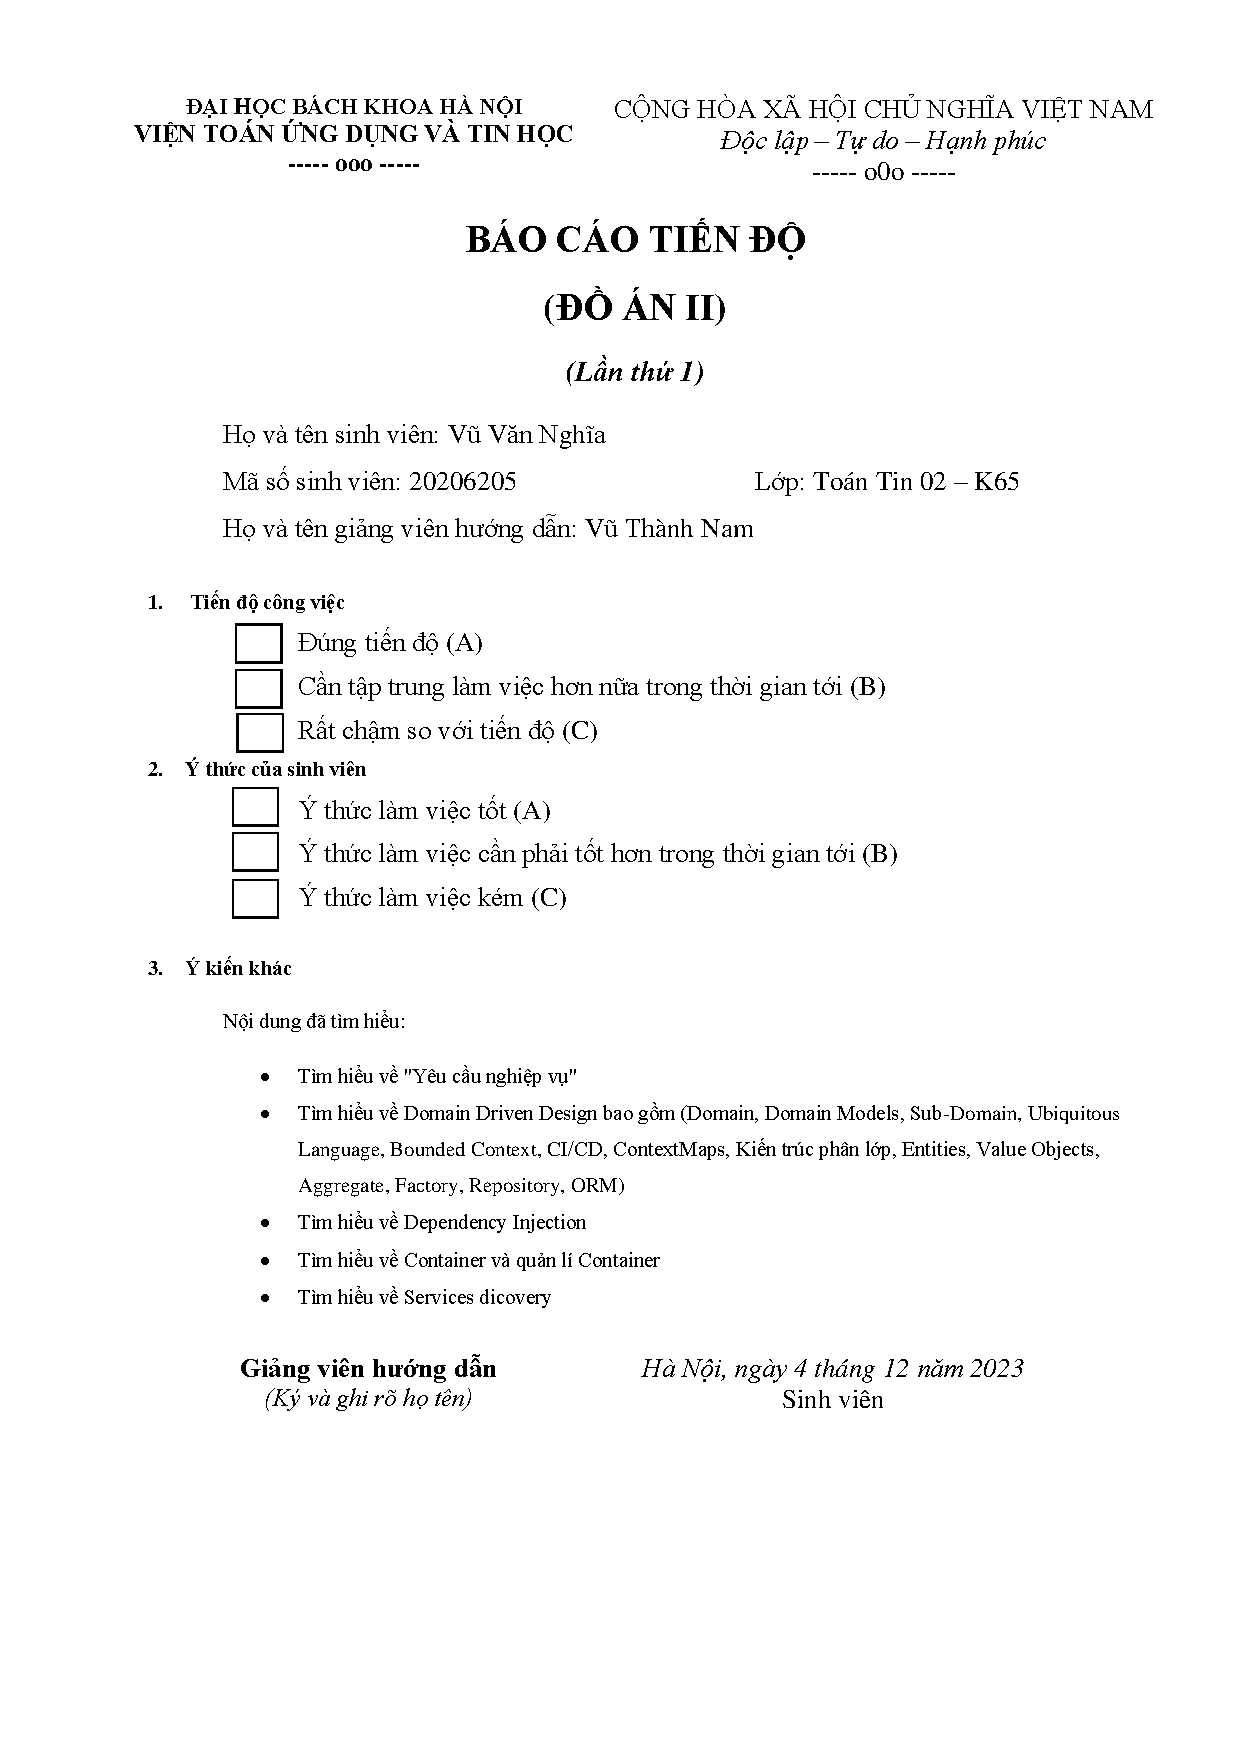
\includepdf[pages = -]{contents/bao_cao_tien_do_1.pdf}

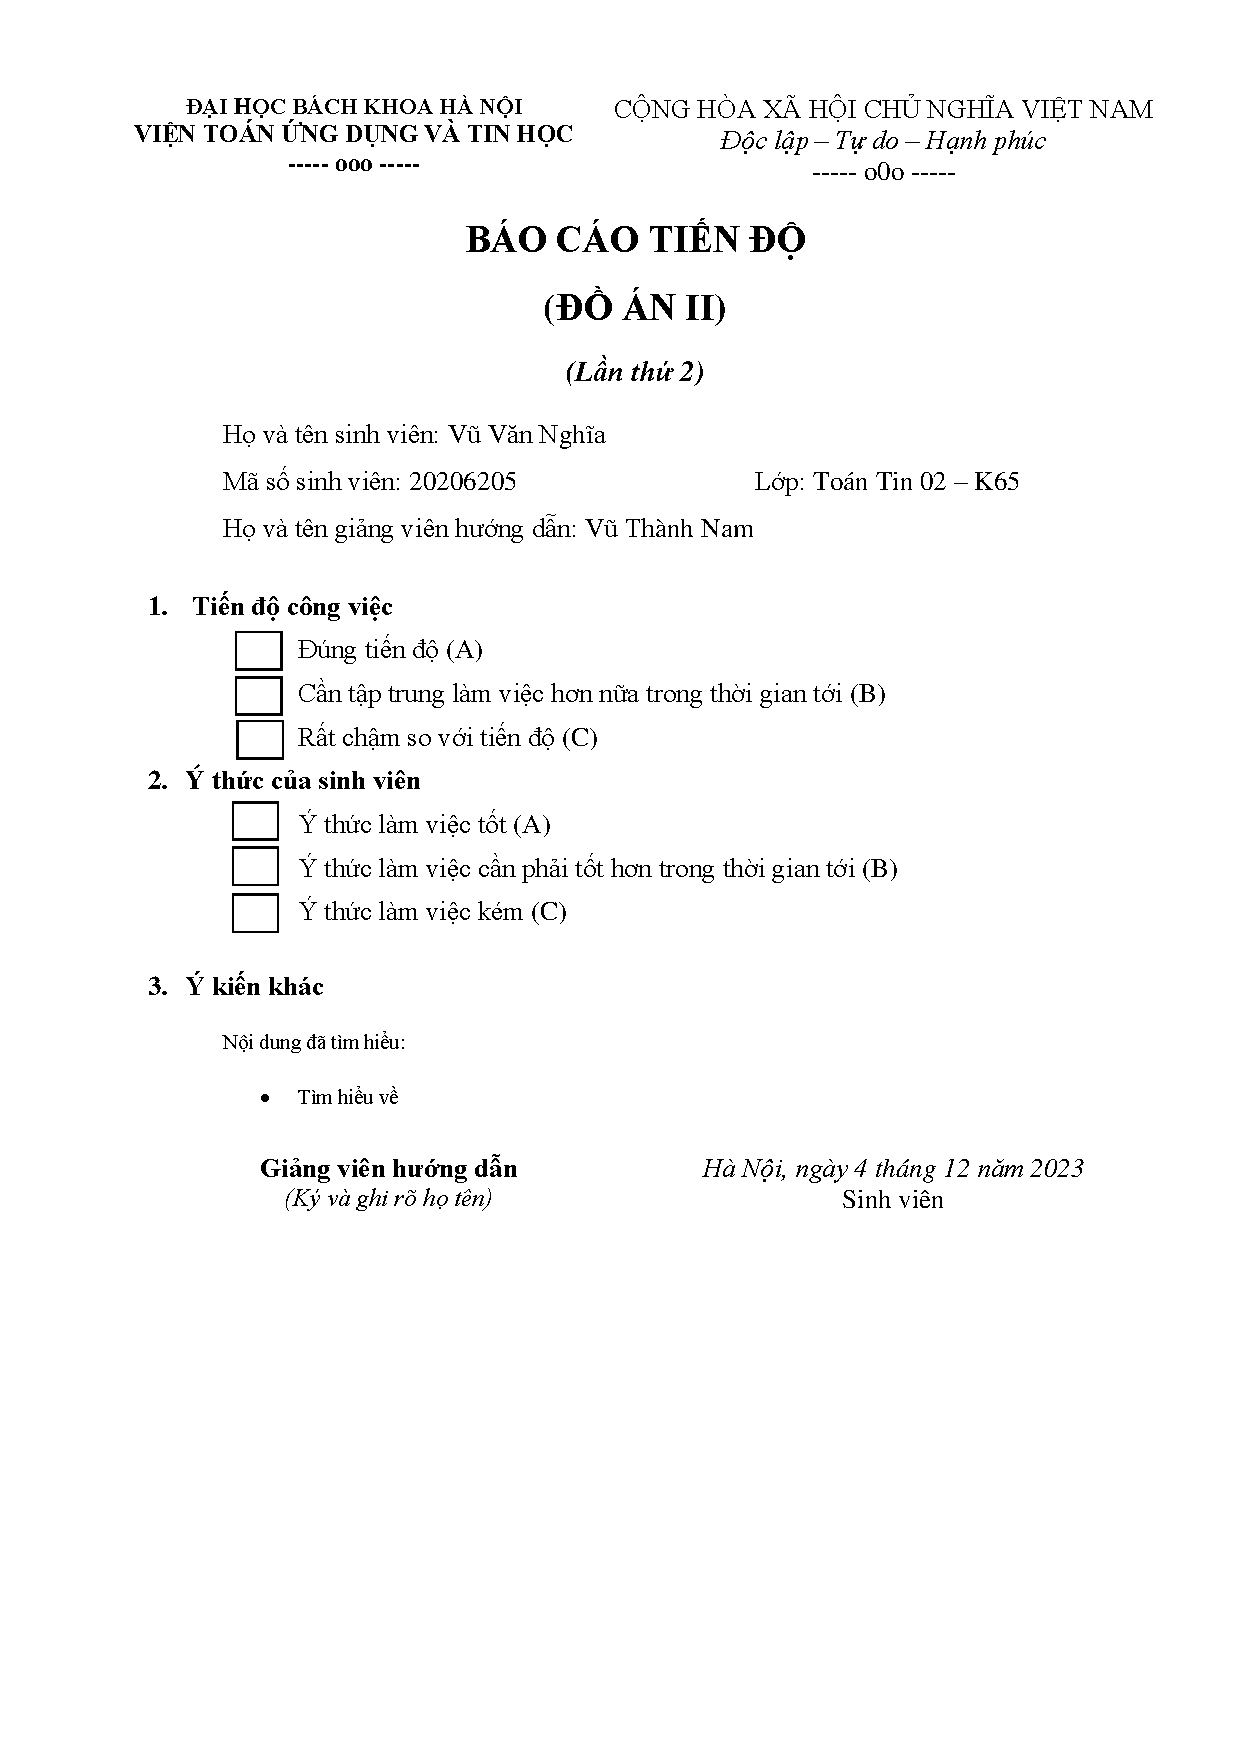
\includepdf[pages = -]{contents/bao_cao_tien_do_2.pdf}

% \end{document} % kết thúc

% Yêu cầu nghiệp vụ của từng sub

% %

% Sơ đồ if else Đ S

% %

% sub trước model

% %

%%%%%%%%%%%%%%%%%%%%%%%%%%%%%%%%%%%%%

\end{document}

\section{xxxxxxx}

\subsection{xxxxxxx}

\subsubsection{xxxxxxx}


\begin{titlepage}

% Vẽ hình chữ nhật

\begin{tikzpicture}[remember picture, overlay]\draw [line width = 3pt]($ (current page.north west) + (3.0cm, - 2.5cm)$)rectangle($ (current page.south east) + (- 2.5cm, 2.5cm)$);\draw [line width = 0.5pt]($ (current page.north west) + (3.1cm, - 2.6cm)$)rectangle($ (current page.south east) + (- 2.6cm, 2.6cm)$);\end{tikzpicture}

\begin{center}

\vspace{- 0.4cm}

\textbf{ĐẠI HỌC BÁCH KHOA HÀ NỘI} \\

\textbf{VIỆN TOÁN ỨNG DỤNG VÀ TIN HỌC} \\

\textbf{******}

\vspace{0.8cm}

\begin{figure}[H]

\centering


\includegraphics[scale = 0.5]{pictures/hust/main.png}

\end{figure}

\vspace{0.7cm}

\textbf{\fontsize{16pt}{30pt}\selectfont {BÁO CÁO ĐỒ ÁN II}}

\vspace{1cm}

\textbf{\fontsize{16pt}{30pt}\selectfont {ĐỀ TÀI:}} \\

\textbf{\fontsize{20pt}{24pt}\selectfont {Sử dụng thiết kế hướng miền \\ xây dựng kiến trúc vi dịch vụ cho \\ bài toán hóa đơn điện tử}} \\

\end{center}

\vspace{0.3cm}

\begin{center}

\textbf{\fontsize{10pt}{24pt}\selectfont {Chuyên ngành: Toán Tin}}

\end{center}

\vspace{0.7cm}

\hspace{3cm}\begin{minipage}{0.7\textwidth}

\begin{tabular}{l l l}

\textbf{\fontsize{10pt}{24pt}\selectfont {Giảng viên hướng dẫn}} & \textbf{\fontsize{10pt}{24pt}\selectfont {TS. Vũ Thành Nam}} \\

\textbf{\fontsize{10pt}{24pt}\selectfont {Sinh viên thực hiện}} & \textbf{\fontsize{10pt}{24pt}\selectfont {Vũ Văn Nghĩa}} \\

\textbf{\fontsize{10pt}{24pt}\selectfont {Mã số sinh viên}} & \textbf{\fontsize{10pt}{24pt}\selectfont {20206205}} \\

\textbf{\fontsize{10pt}{24pt}\selectfont {Lớp}} & \textbf{\fontsize{10pt}{24pt}\selectfont {Toán Tin 02 - K65}} \\

\end{tabular}

\end{minipage}

\vfill

\begin{center}

\textbf{Hà Nội, \the\year}

% \textbf{Hà Nội, \the\month~/~\the\year}

% \textbf{Hà Nội, \the\month~-~\the\year}

\end{center}

\end{titlepage}



\begin{titlepage}

% Vẽ hình chữ nhật

\begin{tikzpicture}[remember picture, overlay]\draw [line width = 3pt]($ (current page.north west) + (3.0cm, - 2.5cm)$)rectangle($ (current page.south east) + (- 2.5cm, 2.5cm)$);\draw [line width = 0.5pt]($ (current page.north west) + (3.1cm, - 2.6cm)$)rectangle($ (current page.south east) + (- 2.6cm, 2.6cm)$);\end{tikzpicture}

\begin{center}

\vspace{- 0.4cm}

\textbf{ĐẠI HỌC BÁCH KHOA HÀ NỘI} \\

\textbf{VIỆN TOÁN ỨNG DỤNG VÀ TIN HỌC} \\

\textbf{******}

\vspace{0.8cm}

\begin{figure}[H]

\centering


\includegraphics[scale = 0.5]{pictures/hust/main.png}

\end{figure}

\vspace{0.7cm}

\textbf{\fontsize{16pt}{30pt}\selectfont {BÁO CÁO ĐỒ ÁN II}}

\vspace{1cm}

\textbf{\fontsize{16pt}{30pt}\selectfont {ĐỀ TÀI:}} \\

\textbf{\fontsize{20pt}{24pt}\selectfont {Sử dụng thiết kế hướng miền \\ xây dựng kiến trúc vi dịch vụ cho \\ bài toán hóa đơn điện tử}} \\

\end{center}

\vspace{0.3cm}

\begin{center}

\textbf{\fontsize{10pt}{24pt}\selectfont {Chuyên ngành: Toán Tin}}

\end{center}

\vspace{0.7cm}

\hspace{3cm}\begin{minipage}{0.7\textwidth}

\begin{tabular}{l l l}

\textbf{\fontsize{10pt}{24pt}\selectfont {Giảng viên hướng dẫn}} & \textbf{\fontsize{10pt}{24pt}\selectfont {TS. Vũ Thành Nam}} \\

\textbf{\fontsize{10pt}{24pt}\selectfont {Sinh viên thực hiện}} & \textbf{\fontsize{10pt}{24pt}\selectfont {Vũ Văn Nghĩa}} \\

\textbf{\fontsize{10pt}{24pt}\selectfont {Mã số sinh viên}} & \textbf{\fontsize{10pt}{24pt}\selectfont {20206205}} \\

\textbf{\fontsize{10pt}{24pt}\selectfont {Lớp}} & \textbf{\fontsize{10pt}{24pt}\selectfont {Toán Tin 02 - K65}} \\

\end{tabular}

\end{minipage}

\vfill

\begin{center}

\textbf{Hà Nội, \the\year}

% \textbf{Hà Nội, \the\month~/~\the\year}

% \textbf{Hà Nội, \the\month~-~\the\year}

\end{center}

\end{titlepage}



\begin{center}

{\bfseries NHẬN XÉT CỦA GIẢNG VIÊN HƯỚNG DẪN}

\end{center}

\begin{enumerate}

\item Mục đích và nội dung của đồ án:

\vspace{20ex}

\item Kết quả đạt được:

\vspace{20ex}

\item Ý thức làm việc của sinh viên:

\vspace{20ex}

\end{enumerate}

\hspace{0.4\textwidth}\begin{minipage}{0.5\textwidth}

\noindent\begin{center}

\textit{Hà Nội, \today} \\

\textbf{Giảng viên hướng dẫn} \\

\textit{(Ký và ghi rõ họ tên)}

\vspace{2cm}

\textbf{TS. Vũ Thành Nam}

\end{center}

\end{minipage}

\pagestyle{empty}



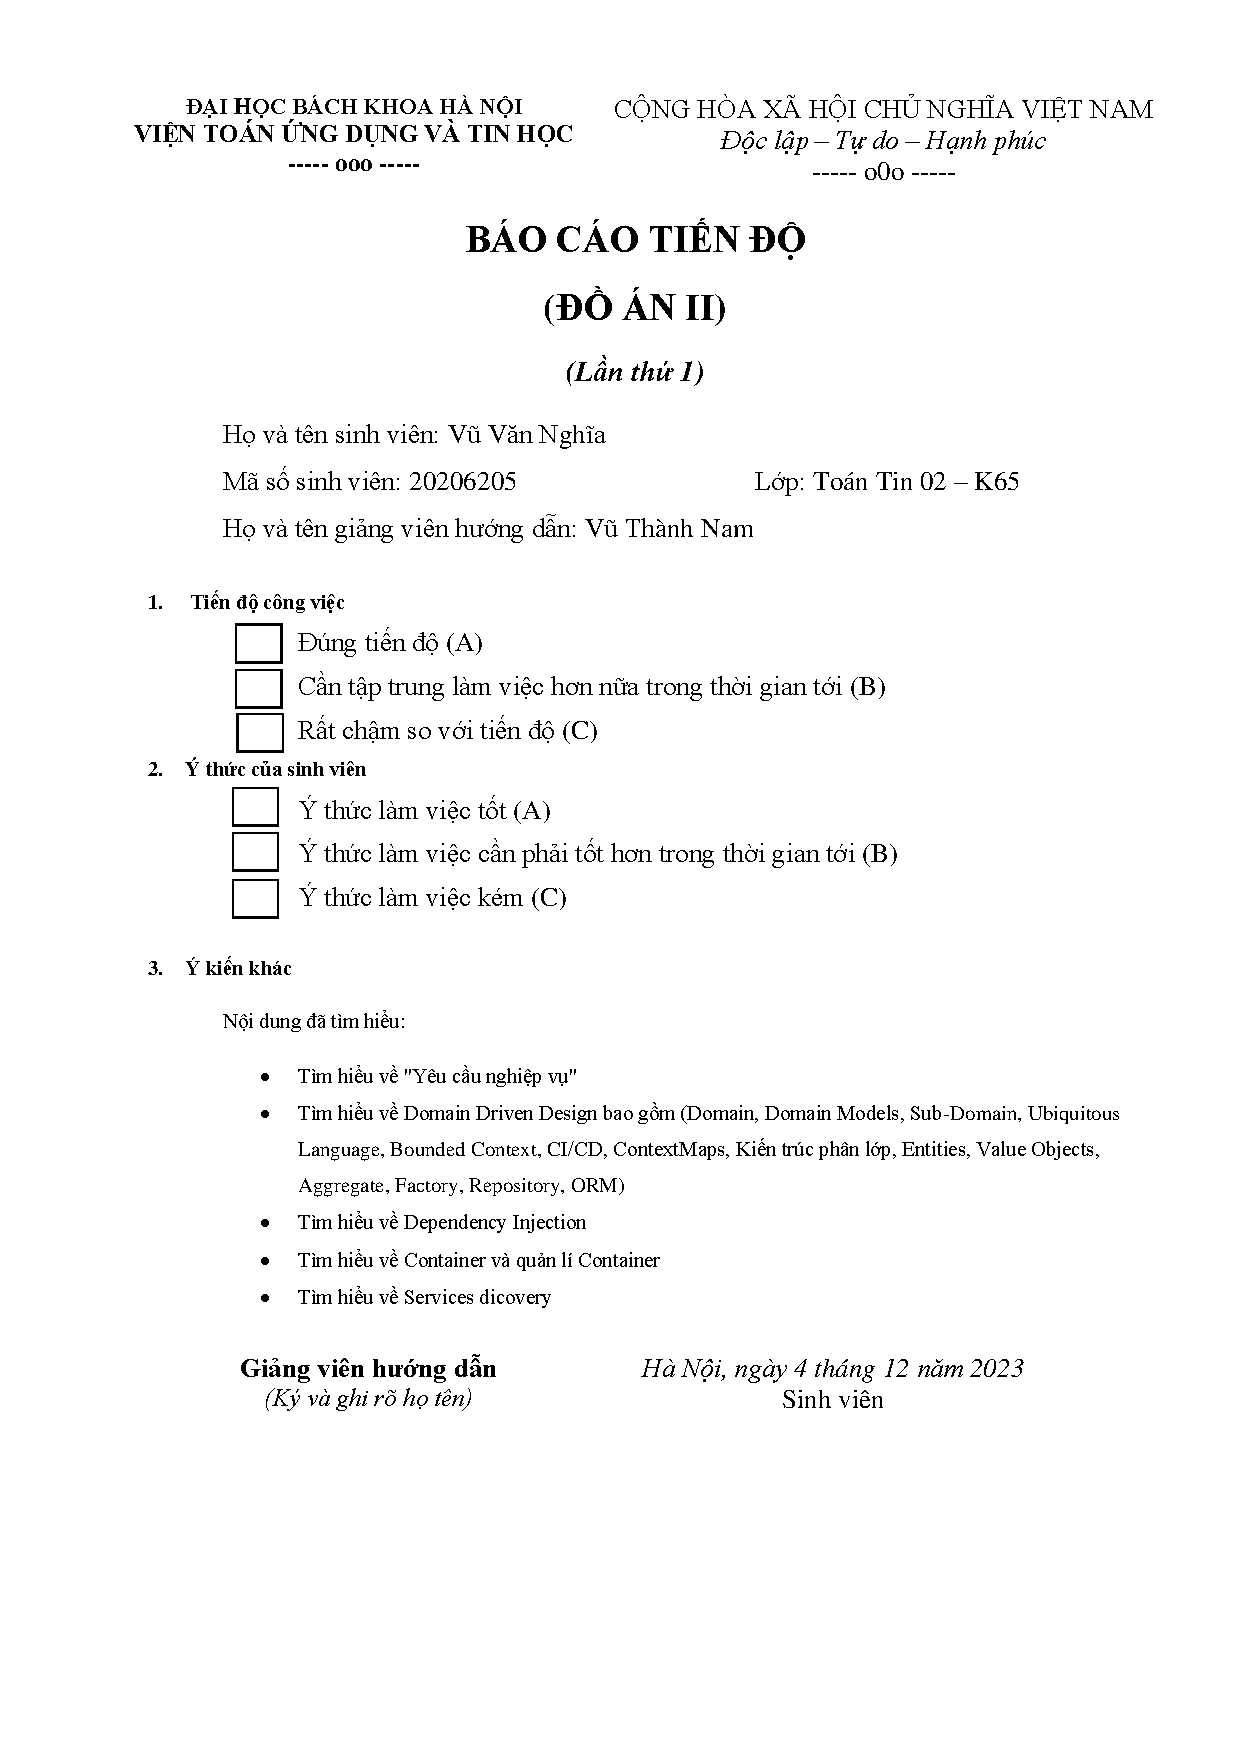
\includepdf[pages = -]{contents/bao_cao_tien_do_1.pdf}

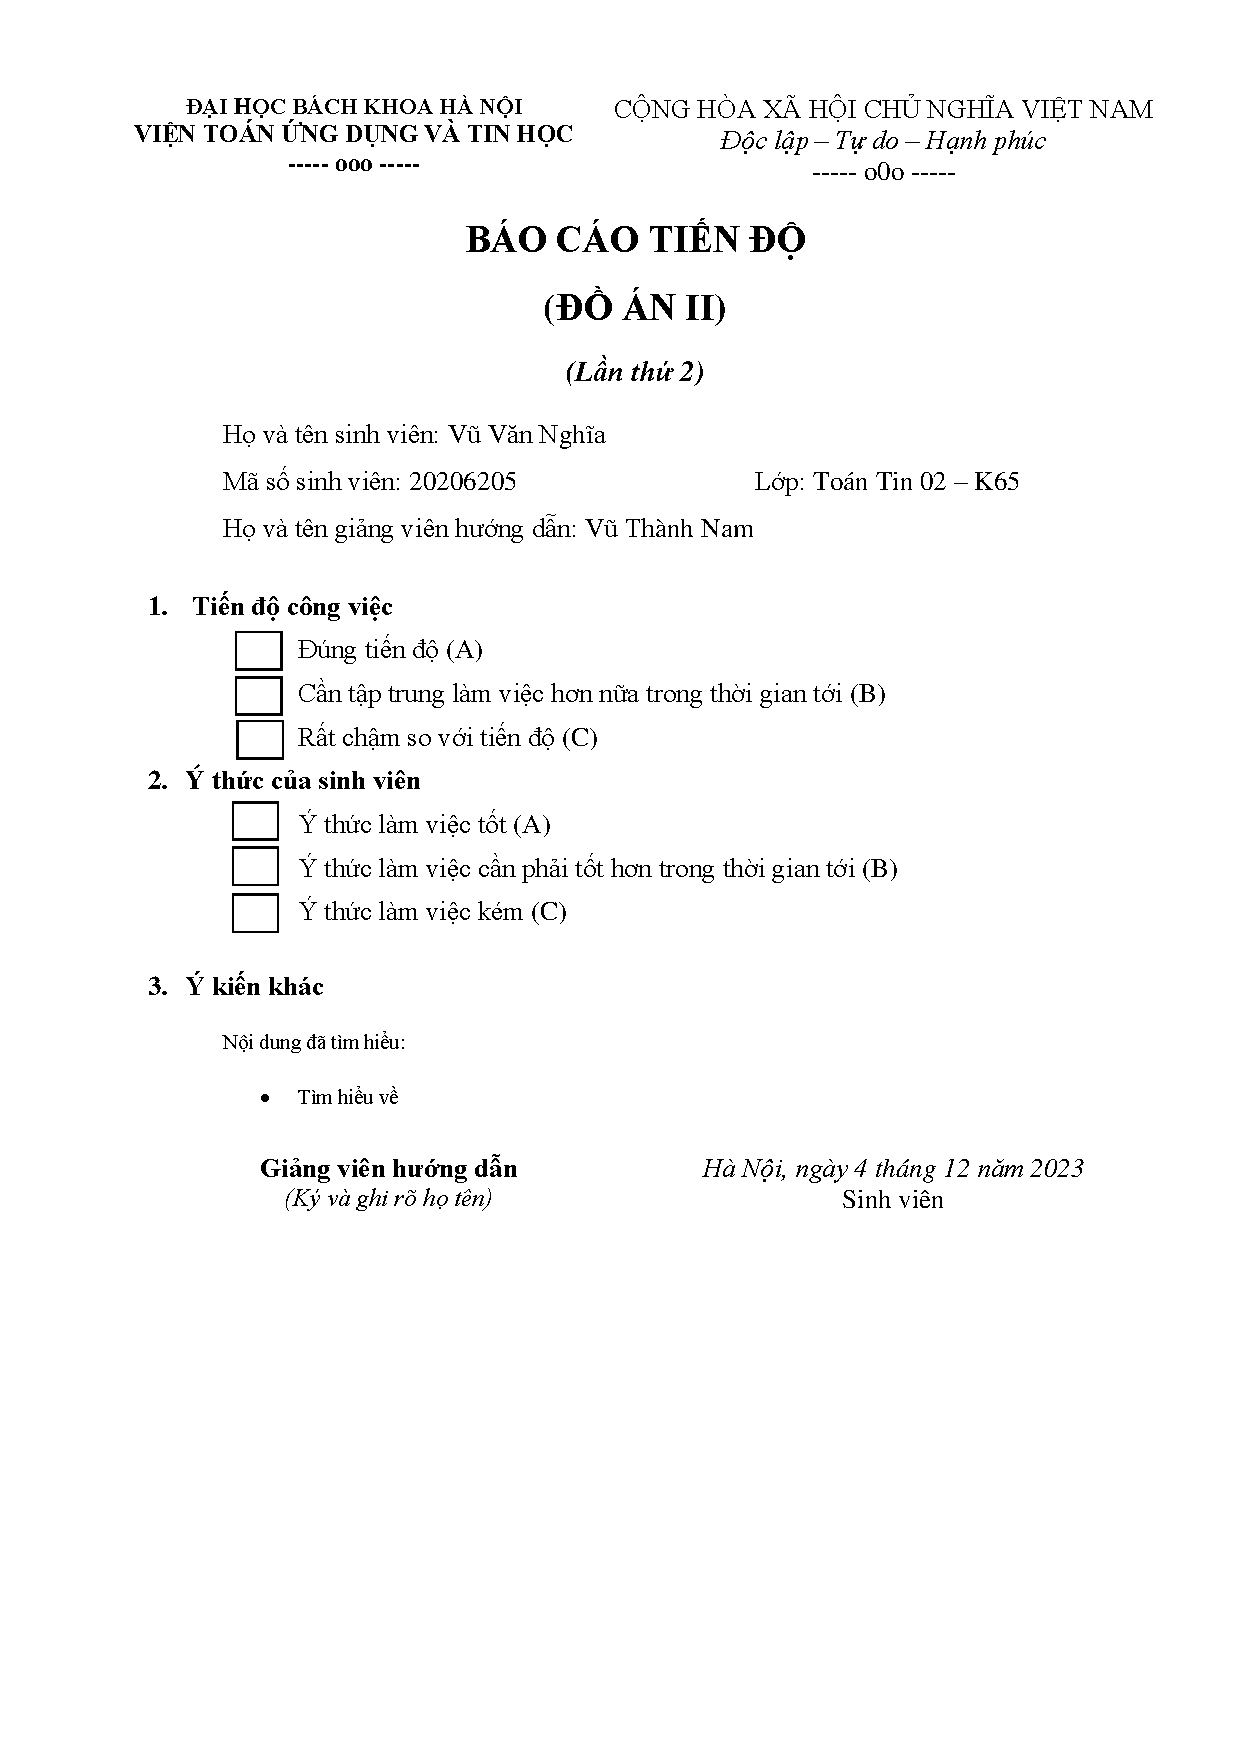
\includepdf[pages = -]{contents/bao_cao_tien_do_2.pdf}

